% !TeX root = ../../Book3.tex
% 纲要标题：## 第2章　测地线、距离、完备性与割迹
% 纲要位置：几何学计划纲要.md，第 2157 行。
% 正文状态：初稿；尚未正式审核。

% 纲要内容开始
% 
% > 本章目标与证明范围：把局部常微分方程、法邻域极小性和整体完备性连续建立。割点与共轭点的精细关系在 Jacobi 理论后再深化；本章不提前使用指标定理。
% 
% 纲要内容结束

\chapter{测地线、距离、完备性与割迹}
\label{g3:ch:02}
\BookChapterNumber{g3:ch:02}

\begin{chapterabstract}
	联络给出测地线方程，长度则给出端点间的内在距离。本章先用常微分方程构造指数映射，由 Gauss 引理证明短径向测地线最短，并建立法坐标与强凸邻域；随后完整证明 Hopf--Rinow 定理，将度量完备、测地线延拓和闭有界集紧性联系起来。最后沿每个初方向定义割时与割迹，说明最短线何时失去唯一性，证明紧集上的注入半径有正下界，并在球面、平坦环面和实射影空间中计算这些量。
\end{chapterabstract}

\begin{learninggoals}
	\begin{itemize}
		\item 从测地线初值问题构造指数映射，说明其定义域、光滑性、零处微分和仿射缩放性质。
		\item 证明 Gauss 引理、径向极小性和强凸邻域存在性，并区分法邻域、短线唯一性与全局最短线。
		\item 逐步完成 Hopf--Rinow 定理的等价闭环，辨认有限维、连通和无边界条件在证明中的用途。
		\item 用割时记录最大极小区间，计算标准模型的割迹与注入半径，比较局部坐标尺度和整体完备性。
	\end{itemize}
\end{learninggoals}

站在球面上一点，指定初始方向后沿大圆匀速前进，运动规律始终不变；到达对径点后，继续沿原方向走却会比回头走更长。这个例子把三个问题分开：初值是否确定一条曲线，这条曲线能否一直延长，以及它的某一段是否在所有连接端点的曲线中最短。第一个问题由微分方程回答，后两个则要结合长度与整体空间来研究。

\ProseParagraphBreak

本章从上一章的 Levi-Civita 联络出发，将“加速度为零”写成切丛上的一阶方程。第一卷第13.1节的最大局部流定理负责存在唯一性与初值依赖，第11.3节的逆函数定理把指数映射变成局部坐标。随后所有关于长度极小性、距离拓扑、凸邻域和完备性的结论都在本章证明。商空间模型还使用第一卷第5.3节的覆盖道路提升；需要时会说明覆盖和局部等距条件。

\ProseParagraphBreak

以下流形均为有限维、Hausdorff、第二可数的光滑流形，度量光滑且正定。除专门的边界反例外，流形无边界；涉及有限值内在距离时取连通流形。局部指数映射的构造不要求完备，只有到讨论整体延拓与割迹时才增加相应假设。可对照 Petersen 第3版第5.2--5.3节、第5.5.1--5.5.3节，以及第5.7.1节、第5.7.3--5.7.4节阅读测地线、距离、指数坐标、完备性与注入半径\cite[第5.2--5.3节; 第5.5.1--5.5.3节; 第5.7.1节; 第5.7.3--5.7.4节]{Petersen2016}。

% !TeX root = ../../Book3.tex
% 纲要标题：### 2.1 指数映射与法坐标
% 纲要位置：几何学计划纲要.md，第 2161 行。
% 正文状态：初稿；尚未正式审核。

% 纲要内容开始
% 
% * 测地线方程及初值依赖
% * 指数映射的微分
% * Gauss 引理的变分证明
% * 法坐标中的度量与联络
% * 局部径向极小性
% 
% 纲要内容结束

\section{指数映射与法坐标}
\label{g3:sec:0201}

在 Euclid 空间中，从点 \(p\) 沿初速度 \(v\) 直行，时间 \(t\) 后到达 \(p+tv\)。这既确定一条曲线，也把原点附近的向量变成 \(p\) 附近的点。在黎曼流形上，“速度不改变”应写成速度沿自身的协变导数为零。先解这一初值问题，再把时间一的终点作为向量的像，就得到指数映射。它在零向量附近可逆，由此产生的坐标使从中心出发的测地线成为直线；这些曲线的长度极小性还需要度量的进一步分析。

\subsection{测地线方程及初值依赖}
\label{g3:subsec:0201:01}

设 \(\gamma:I\to M\) 为光滑曲线，\(V(t)\in\mathrm{T}_{\gamma(t)}M\) 为沿曲线的光滑向量场。在坐标中写 \(\gamma(t)=(x^i(t))\)、\(V(t)=V^k(t)\partial_k|_{\gamma(t)}\)，沿曲线的协变导数为
\begin{equation}\label{g3:eq:covariant-derivative-along-curve}
	\mathrm{D}_tV
	=\left(\dot V^k+\Gamma^k_{ij}(x(t))\dot x^iV^j\right)\partial_k.
\end{equation}
这是把式\eqref{g3:eq:coordinate-covariant-derivative}限制到曲线后的表达；向量场沿曲线的分量可以独立指定，不要求先在曲线像的邻域上延拓。上一章的 Christoffel 换坐标公式保证这个表达在交叠处一致。度量相容性给出
\[
	\frac{\mathrm{d}}{\mathrm{d}t}g(V,W)
	=g(\mathrm{D}_tV,W)+g(V,\mathrm{D}_tW).
\]

\begin{definition}\label{g3:def:geodesic}
	设 \((M,g)\) 为无边界光滑黎曼流形，\(\nabla\) 为其 Levi-Civita 联络。若光滑曲线 \(\gamma:I\to M\) 满足 \(\mathrm{D}_t\dot\gamma=0\)，则称 \(\gamma\) 为\term[cedixian]{测地线}[geodesic]。常值曲线也包括在内。坐标中的测地线方程是
	\begin{equation}\label{g3:eq:geodesic-equation}
		\ddot x^k+\Gamma^k_{ij}(x)\dot x^i\dot x^j=0,
		\qquad k=1,\ldots,n.
	\end{equation}
\end{definition}

这是一组二阶方程，所以初值同时包括位置 \(p\) 与速度 \(v\in\mathrm{T}_pM\)。把速度也作为未知量，令 \(v^i=\dot x^i\)，就得到切丛坐标 \((x^i,v^i)\) 中的一阶系统
\[
	\dot x^k=v^k,\qquad
	\dot v^k=-\Gamma^k_{ij}(x)v^iv^j.
\]
其右端定义切丛上的光滑向量场
\begin{equation}\label{g3:eq:geodesic-spray}
	S=v^i\frac{\partial}{\partial x^i}
	-\Gamma^k_{ij}(x)v^iv^j\frac{\partial}{\partial v^k}.
\end{equation}
称其为\term[cedixianpenwu]{测地线喷雾}[geodesic spray]。换坐标时，速度分量按 \(\widetilde v^a=(\partial y^a/\partial x^i)v^i\) 变换；对此求时间导数产生的二阶坐标导数，恰与 Christoffel 变换中的二阶项抵消。因此各图中的 \(S\) 表示同一个切丛向量场。它的积分曲线正是 \((\gamma(t),\dot\gamma(t))\)。

\begin{theorem}\label{g3:thm:geodesic-ivp}
	设 \((M,g)\) 为有限维、Hausdorff、第二可数、无边界的光滑黎曼流形。对每个 \(p\in M\)、\(v\in\mathrm{T}_pM\)，存在唯一的最大测地线
	\[
		\gamma_{p,v}:I_{p,v}\longrightarrow M,\qquad
		\gamma_{p,v}(0)=p,\quad \dot\gamma_{p,v}(0)=v,
	\]
	其中 \(I_{p,v}\) 为含零的开区间，任意同初值测地线都是它的限制。集合
	\[
		\mathcal D=\{(t,p,v):v\in\mathrm{T}_pM,\ t\in I_{p,v}\}
		\subset\mathbb R\times\mathrm{T}M
	\]
	开，映射 \((t,p,v)\mapsto(\gamma_{p,v}(t),\dot\gamma_{p,v}(t))\) 在其上光滑。每条测地线速度的长度恒为 \(|v|_g\)。当 \(v=0\) 时，测地线恒为 \(p\)，且 \(I_{p,0}=\mathbb R\)；当 \(a\ne0\) 时，
	\begin{equation}\label{g3:eq:geodesic-scaling}
		I_{p,av}=a^{-1}I_{p,v},\qquad
		\gamma_{p,av}(t)=\gamma_{p,v}(at).
	\end{equation}
	任意仿射重参数 \(t=as+b\) 仍给出测地线。
\end{theorem}
\begin{proof}
	第一卷第13.1节“最大局部流”定理说明：无边界、有限维、Hausdorff、第二可数光滑流形上的光滑向量场，有唯一的最大积分曲线；它们的时间与初值组成开定义域，解映射在该定义域上联合光滑。切丛 \(\mathrm{T}M\) 是满足这些条件的 \(2n\) 维流形，而式\eqref{g3:eq:geodesic-spray}给出其上的光滑向量场。因此该定理适用于 \(S\)。其积分曲线的第一组方程保证第二分量是第一分量的速度，第二组方程正是测地线方程，故得到存在、唯一、最大区间及光滑依赖。
	% 跨卷依赖：g1:thm:maximal-local-flow，已核读其陈述与证明。

	由度量相容性，
	\[
		\frac{\mathrm{d}}{\mathrm{d}t}|\dot\gamma|_g^2
		=2g(\mathrm{D}_t\dot\gamma,\dot\gamma)=0,
	\]
	所以速度长度为常数。零初值速度给出常曲线，唯一性使它就是最大解。

	若 \(a\ne0\)，曲线 \(t\mapsto\gamma_{p,v}(at)\) 的协变加速度是原曲线协变加速度的 \(a^2\) 倍，且初速度为 \(av\)，故它是相应初值解。最大性先给出 \(a^{-1}I_{p,v}\subset I_{p,av}\)；再用缩放因子 \(a^{-1}\) 得反向包含，证明式\eqref{g3:eq:geodesic-scaling}。同一求导计算允许时间平移，因而仿射重参数保持测地线方程。
\end{proof}

对于非恒定测地线，参数中的“匀速”是方程的一部分。若以光滑函数 \(t=h(s)\) 重参数，则
\[
	\mathrm{D}_s\frac{\mathrm{d}}{\mathrm{d}s}\gamma(h(s))
	=h''(s)\dot\gamma(h(s)).
\]
原速度处处非零，因此新曲线仍满足测地线方程当且仅当 \(h''=0\)。曲线的像可以不变，所用参数却未必仍是测地线参数。

\subsection{指数映射的微分}
\label{g3:subsec:0201:02}

初速度的大小同时记录了单位时间内走多远。由缩放公式，沿速度 \(v\) 运动时间 \(t\)，与沿速度 \(tv\) 运动时间一到达同一点。于是可以把时间固定，将所有允许的初速度组织成一个映射。

\begin{definition}\label{g3:def:exponential-map}
	设 \((M,g)\) 为光滑无边界黎曼流形。定义
	\[
		\mathcal E=\{(p,v)\in\mathrm{T}M:1\in I_{p,v}\},
		\qquad
		\mathcal E_p=\mathcal E\cap\mathrm{T}_pM.
	\]
	映射
	\[
		\operatorname{Exp}:\mathcal E\longrightarrow M,\qquad
		\operatorname{Exp}(p,v)=\gamma_{p,v}(1)
	\]
	称为\term[zhishuyingshe]{指数映射}[exponential map]，其在单个切空间上的限制记为 \(\exp_p:\mathcal E_p\to M\)。
\end{definition}

\begin{proposition}\label{g3:prop:exponential-local}
	设 \((M,g)\) 为有限维、Hausdorff、第二可数、无边界光滑黎曼流形。指数映射的定义域 \(\mathcal E\) 是包含零截面的开集，\(\operatorname{Exp}\) 光滑；每个 \(\mathcal E_p\) 关于零向量星形，即 \(v\in\mathcal E_p\)、\(0\le t\le1\) 时 \(tv\in\mathcal E_p\)。在自然识别 \(\mathrm{T}_0(\mathrm{T}_pM)=\mathrm{T}_pM\) 下，
	\begin{equation}\label{g3:eq:exponential-derivative-zero}
		(\mathrm{d}\exp_p)_0=\operatorname{id}_{\mathrm{T}_pM}.
	\end{equation}
	因此存在 \(R>0\)，使 \(\exp_p\) 在切空间开球 \(B_p(0,R)=\{v:|v|_g<R\}\) 上为到其像的微分同胚。此外，端点映射
	\begin{equation}\label{g3:eq:geodesic-endpoint-map}
		F:\mathcal E\longrightarrow M\times M,\qquad
		F(p,v)=(p,\exp_pv)
	\end{equation}
	在每个 \((p,0)\) 附近为局部微分同胚。
\end{proposition}
\begin{proof}
	\(\mathcal E\) 是开集 \(\mathcal D\) 在时间一的切片，故开；指数映射是测地流在该切片上的位置分量，故光滑。零速度解对所有时间存在，所以 \(\mathcal E\) 包含零截面。若 \(v\in\mathcal E_p\)，开区间 \(I_{p,v}\) 包含 \([0,1]\)。对 \(0<t\le1\)，式\eqref{g3:eq:geodesic-scaling}说明 \(1\in I_{p,tv}\)，而 \(t=0\) 已经处理，故纤维星形。

	任取 \(w\in\mathrm{T}_pM\)。当 \(s\) 充分接近零时，缩放公式给出
	\[
		\exp_p(sw)=\gamma_{p,w}(s).
	\]
	在 \(s=0\) 求导，右侧导数是初速度 \(w\)，便得到式\eqref{g3:eq:exponential-derivative-zero}。第一卷定理11.3.3的逆函数定理适用于同维无边界流形之间微分可逆的光滑映射，因此 \(\exp_p\) 在零向量的某个邻域上为微分同胚。取包含于该邻域的小球，即得所述 \(R\)。
	% 跨卷依赖：g1:thm:inverse-function。

	最后看起点也变化的情形。在零截面处有自然分裂
	\[
		\mathrm{T}_{(p,0)}(\mathrm{T}M)
		\simeq\mathrm{T}_pM\oplus\mathrm{T}_pM:
	\]
	第一项由零截面上移动起点得到，第二项由固定起点、改变纤维向量得到。由于 \(\exp_x0=x\)，第一项对终点的导数是恒等；式\eqref{g3:eq:exponential-derivative-zero}说明第二项也是恒等。故
	\[
		\mathrm{d}F_{(p,0)}(\xi,\eta)=(\xi,\xi+\eta).
	\]
	这个线性映射可逆，逆为 \((\xi,\zeta)\mapsto(\xi,\zeta-\xi)\)。再次应用逆函数定理，得到 \((p,0)\) 和 \((p,p)\) 的开邻域之间的光滑局部逆。
\end{proof}

\begin{definition}\label{g3:def:normal-neighborhood}
	若 \(U\subset\mathcal E_p\) 是包含零、关于零星形的开集，且 \(\exp_p|_U\) 为微分同胚，则称 \(\exp_p(U)\) 为 \(p\) 的\term[falinyu]{法邻域}[normal neighborhood]。当 \(U=B_p(0,R)\) 为球时，称其像为 \(p\) 的\term[faqiu]{法球}[normal ball]。
\end{definition}

这里的球先在切空间中按 \(g_p\) 定义，其像与内在距离球的关系将在长度极小性之后建立。\cref{g3:prop:exponential-local}的端点映射还说明：起点与终点同时作小变化时，连接它们的一个小初速度可以光滑地求出。第二节将据此统一邻近起点可用的半径。

\begin{example}\label{g3:exm:interval-exponential-domain}
	在开区间 \(M=(0,1)\) 上取 \(g=\mathrm{d}x^2\)。测地线是 \(\gamma_{p,v}(t)=p+tv\)，只允许取使其仍落在 \((0,1)\) 的最大时间区间。因此
	\[
		\mathcal E_p=(-p,1-p),\qquad \exp_p(v)=p+v.
	\]
	定义域包含零且星形，却通常不是整个切空间。指数映射局部存在无需整体延拓到所有时间。
\end{example}

\begin{example}\label{g3:exm:round-sphere-exponential}
	半径 \(a>0\) 的圆球面 \(S_a^n\subset\mathbb R^{n+1}\) 取诱导度量。对 \(p\in S_a^n\) 及非零 \(v\in\mathrm{T}_pS_a^n\)，令
	\[
		\gamma(t)=\cos(t|v|/a)p
		+a\sin(t|v|/a)\frac{v}{|v|}.
	\]
	因为 \(p\perp v\)、\(|p|=a\)，这条曲线始终在球面上，初速度为 \(v\)，且 \(\gamma''(t)=-(|v|^2/a^2)\gamma(t)\) 沿法向。由\cref{g3:prop:induced-connection-projection}，其协变加速度为零，所以唯一性给出
	\begin{equation}\label{g3:eq:round-sphere-exponential}
		\exp_p(v)=\cos(|v|/a)p
		+a\frac{\sin(|v|/a)}{|v|}v,
		\qquad \exp_p(0)=p.
	\end{equation}
	右端在零处光滑，因为 \(\cos(|v|/a)\) 和 \(\sin(|v|/a)/|v|\) 都是 \(|v|^2\) 的光滑函数。

	这个映射把 \(B_p(0,\pi a)\) 微分同胚地送到 \(S_a^n\setminus\{-p\}\)。事实上，对既非 \(p\) 又非 \(-p\) 的 \(q\)，令
	\[
		\vartheta=\arccos\frac{\langle p,q\rangle}{a^2}\in(0,\pi),
		\qquad
		u=\frac{q-\cos\vartheta\,p}{a\sin\vartheta}.
	\]
	则 \(u\) 是唯一的单位切向量，使 \(q=\exp_p(a\vartheta u)\)。此逆在远离 \(p\) 处光滑，在 \(p\) 附近与逆函数定理给出的光滑逆一致。半径等于 \(\pi a\) 的所有向量则映到同一个对径点 \(-p\)，显示局部可逆的范围会受到整体几何限制。
\end{example}

\subsection{Gauss 引理的变分证明}
\label{g3:subsec:0201:03}

指数映射把每条径向直线变成测地线。若同时改变初速度的方向，这些测地线便形成一族曲线。比较径向运动与这种横向变化，就可以判断指数映射如何处理正交关系；它也是随后证明长度极小性的依据。这个结论称为 Gauss 引理。\footnote{Carl Friedrich Gauss（1777--1855），德国数学家，在数论、微分几何和测地学等领域作出重要贡献。}

\begin{lemma}[Gauss 引理]\label{g3:lem:gauss}
	设 \((M,g)\) 为光滑无边界黎曼流形，\(p\in M\)，\(v\in\mathcal E_p\)，并用向量空间的平移识别 \(\mathrm{T}_v(\mathrm{T}_pM)=\mathrm{T}_pM\)。对任意 \(w\in\mathrm{T}_pM\)，有
	\begin{equation}\label{g3:eq:gauss-lemma}
		g_{\exp_pv}\bigl((\mathrm{d}\exp_p)_vv,(\mathrm{d}\exp_p)_vw\bigr)
		=g_p(v,w).
	\end{equation}
	特别地，指数映射保持径向向量的长度，并把与 \(v\) 正交的向量送到与径向速度正交的向量。
\end{lemma}
\begin{proof}
	\(v=0\) 时等式两边都为零。以下固定 \(v\ne0\)。由于 \(\mathcal E_p\) 开，可取小参数区间，使 \(v+sw\in\mathcal E_p\)。考虑光滑变分
	\[
		H(s,t)=\exp_p\bigl(t(v+sw)\bigr)=\gamma_{p,v+sw}(t),
		\qquad 0\le t\le1.
	\]
	记沿这个变分的向量场 \(T=\partial_tH\)、\(V=\partial_sH\)。每条 \(t\)-曲线都是测地线，故 \(\mathrm{D}_tT=0\)；又因 \(H(s,0)=p\)，有 \(V(s,0)=0\)。

	先补明混合协变导数为何可以交换。在任一覆盖变分像的坐标图内，
	\[
		(\mathrm{D}_tV)^k
		=\partial_t\partial_sH^k+\Gamma^k_{ij}(H)\partial_tH^i\partial_sH^j,
	\]
	而 \((\mathrm{D}_sT)^k\) 由交换 \(s,t\) 得到。普通混合偏导相等，且无挠性给出 \(\Gamma^k_{ij}=\Gamma^k_{ji}\)，所以
	\begin{equation}\label{g3:eq:mixed-variation-derivatives}
		\mathrm{D}_tV=\mathrm{D}_sT.
	\end{equation}
	这个计算只用光滑映射 \(H\) 的坐标表达，不要求 \(H\) 是浸入，因而也适用于 \(t=0\)。

	由度量相容性和式\eqref{g3:eq:mixed-variation-derivatives}，
	\[
		\partial_t g(T,V)
		=g(T,\mathrm{D}_tV)
		=g(T,\mathrm{D}_sT)
		=\frac12\partial_s g(T,T).
	\]
	每条测地线常速，故 \(g(T,T)=g_p(v+sw,v+sw)\)，与 \(t\) 无关。在 \(s=0\) 处，上式右端就是 \(g_p(v,w)\)。从 \(t=0\) 积分到 \(t=1\)，利用初始内积为零，得到
	\[
		g(T(0,1),V(0,1))=g_p(v,w).
	\]
	链式法则给出 \(T(0,1)=(\mathrm{d}\exp_p)_vv\)、\(V(0,1)=(\mathrm{d}\exp_p)_vw\)，即为所求。取 \(w=v\) 得径向长度保持；取 \(w\perp v\) 得正交关系。
\end{proof}

在法球去掉中心的部分，写 \(v=ru\)，其中 \(|u|_g=1\)、\(r>0\)。定义径向单位向量
\[
	\partial_r\big|_{\exp_p(ru)}=(\mathrm{d}\exp_p)_{ru}u.
\]
Gauss 引理说明其长度为一，并与固定半径的球面像正交。因此在这些极坐标中，度量可以写成
\[
	g=\mathrm{d}r^2+g_r,
\]
其中 \(g_r\) 是单位方向球面上的一族正定度量。这里 \(g_r\) 随 \(r\) 及方向变化，中心 \(r=0\) 则应使用下面的光滑法坐标。

\subsection{法坐标中的度量与联络}
\label{g3:subsec:0201:04}

在 \(\mathrm{T}_pM\) 选一组 \(g_p\)-正交单位基 \((E_1,\ldots,E_n)\)。把法球中的点写成
\[
	q=\exp_p(x^iE_i),
\]
便得到以 \(p\) 为中心的\term[fazuobiao]{法坐标}[normal coordinates] \(x^1,\ldots,x^n\)。这些坐标先在切空间中作线性坐标，再经指数映射送到流形；它们的特殊性来自径向直线恰好成为测地线。

\begin{proposition}\label{g3:prop:normal-coordinate-first-order}
	设 \((M,g)\) 为光滑无边界黎曼流形，在 \(p\) 的法邻域中采用由 \(g_p\)-正交单位基产生的法坐标。则在中心 \(p\)，
	\begin{equation}\label{g3:eq:normal-coordinate-first-order}
		g_{ij}(p)=\delta_{ij},\qquad
		\Gamma^k_{ij}(p)=0,\qquad
		\partial_k g_{ij}(p)=0.
	\end{equation}
\end{proposition}
\begin{proof}
	由 \((\mathrm{d}\exp_p)_0=\operatorname{id}\)，有 \(\partial_i|_p=E_i\)，故 \(g_{ij}(p)=\delta_{ij}\)。对任意 \(a=(a^1,\ldots,a^n)\)，曲线 \(t\mapsto\exp_p(ta^iE_i)\) 在足够小时间内是测地线，其法坐标为 \(x^i(t)=ta^i\)。在 \(t=0\) 将它代入测地线方程，得到
	\[
		\Gamma^k_{ij}(p)a^ia^j=0\qquad\text{对一切 }a.
	\]
	先取 \(a\) 为单个坐标基向量，再取两个坐标基向量的和，并用 \(\Gamma^k_{ij}=\Gamma^k_{ji}\)，便得到所有系数都为零。最后，度量相容性写成
	\[
		\partial_k g_{ij}
		=\Gamma^\ell_{ki}g_{\ell j}+\Gamma^\ell_{kj}g_{i\ell};
	\]
	在 \(p\) 求值就得到度量的一阶偏导全部为零。
\end{proof}

所以在中心附近，Taylor 公式给出 \(g_{ij}(x)=\delta_{ij}+O(|x|^2)\)。法坐标消去了中心处的一阶度量变化；二阶及更高阶变化仍记录实际几何。第三章将把二阶项与曲率联系起来。极坐标中的 \(\mathrm{d}r^2+g_r\) 和这里的 \(g_{ij}(x)\) 描述同一度量：前者突出径向正交性，后者在中心仍保持光滑。

\subsection{局部径向极小性}
\label{g3:subsec:0201:05}

考虑从法球中心 \(p\) 走到 \(q=\exp_p(v)\)。径向测地线长度为 \(|v|_g\)。沿其他曲线前进时，速度可以分成径向分量和球面方向分量；Gauss 引理使两部分正交，因此球面方向的运动会增加总长度。还须处理一个整体问题：竞争曲线可能先离开法球，再从外面绕回 \(q\)。缩小一层法球后，首次离开所付出的长度足以排除这种捷径。

\begin{proposition}\label{g3:prop:normal-radial-minimality}
	设 \((M,g)\) 为有限维、Hausdorff、第二可数、无边界光滑黎曼流形，\(p\in M\)、\(R>0\)，并设 \(\exp_p:B_p(0,R)\to U_R\) 为微分同胚。则有以下结论。
	\begin{enumerate}
		\item 对 \(v\in B_p(0,R)\)，从 \(p\) 到 \(q=\exp_pv\) 的任意连续分片 \(C^1\) 曲线 \(c:[a,b]\to M\) 都满足
		\[
			L_g(c)\ge |v|_g.
		\]
		径向测地线 \(t\mapsto\exp_p(tv)\)、\(0\le t\le1\)，达到这个下界。
		\item 若 \(v\ne0\)，等号成立当且仅当
		\[
			c(t)=\exp_p(\lambda(t)v),
		\]
		其中 \(\lambda:[a,b]\to[0,1]\) 为非减的连续分片 \(C^1\) 函数，\(\lambda(a)=0\)、\(\lambda(b)=1\)。因此允许停顿时，最短曲线的像仍是唯一的径向线段；固定参数区间及常速后，曲线也唯一。
		\item 对任意 \(0<r<R\)，曲线从 \(p\) 首次到达 \(U_r=\exp_p(B_p(0,r))\) 的边界时，已经走过的长度至少为 \(r\)。集合 \(\overline{U_r}=\exp_p(\overline{B_p(0,r)})\) 紧。
	\end{enumerate}
\end{proposition}
\begin{proof}
	先在 \(U_R\) 内比较长度。令 \(x(t)=\exp_p^{-1}(c(t))\)、\(\rho(t)=|x(t)|_g\)。在 \(x(t)\ne0\) 处，Gauss 引理与内积不等式给出
	\[
		|\dot\rho(t)|
		=\left|g\left((\mathrm{d}\exp_p)_{x(t)}
			\frac{x(t)}{|x(t)|_g},\dot c(t)\right)\right|
		\le|\dot c(t)|_g.
	\]
	曲线经过 \(p\) 时，\(\rho\) 未必可微。为直接处理这些时刻，取
	\[
		\rho_\varepsilon(t)=\sqrt{|x(t)|_g^2+\varepsilon^2},
		\qquad\varepsilon>0.
	\]
	它在每个 \(C^1\) 片段上都是 \(C^1\)。在 \(x\ne0\) 处，其导数为 \(\rho/\sqrt{\rho^2+\varepsilon^2}\) 乘以 \(\dot\rho\)；在 \(x=0\) 处，直接求导得零。因此处处有 \(|\dot\rho_\varepsilon|\le|\dot c|_g\)。逐片积分并令 \(\varepsilon\to0\)，对任意子区间 \([s,t]\) 得到
	\begin{equation}\label{g3:eq:radial-length-bound}
		L_g(c|_{[s,t]})\ge|\rho(t)-\rho(s)|.
	\end{equation}
	这个论证也包括速度为零和多次经过中心的曲线。

	再排除离开法球的竞争曲线。固定 \(|v|_g<r<R\)。闭切球 \(\overline{B_p(0,r)}\) 紧，其像 \(K_r\) 紧，因 \(M\) 为 Hausdorff 空间而闭；又因 \(\exp_p\) 在更大的开球上为微分同胚，\(K_r\) 的内部是 \(U_r\)，边界是半径 \(r\) 的切球面之像。因此 \(K_r=\overline{U_r}\subset U_R\)。若 \(c\) 离开 \(U_r\)，连续性给出首次到达边界的时刻 \(\tau\)，且 \(c([a,\tau])\subset K_r\)。这段曲线可在 \(U_R\) 中提升，式\eqref{g3:eq:radial-length-bound}给出
	\[
		L_g(c)\ge L_g(c|_{[a,\tau]})\ge r>|v|_g.
	\]
	若 \(c\) 始终在 \(U_r\) 中，直接用式\eqref{g3:eq:radial-length-bound}得到 \(L_g(c)\ge|v|_g\)。径向测地线的速度长度恒为 \(|v|_g\)，故在时间区间 \([0,1]\) 上恰有此长度。这也证明了第三项。

	最后分析等号。设 \(v\ne0\) 且 \(L_g(c)=|v|_g\)。刚才的严格不等式保证曲线始终在 \(U_r\) 中。对任意 \(a\le s\le t\le b\)，分别对三段使用式\eqref{g3:eq:radial-length-bound}，并考虑有向径向变化，得到
	\[
		\begin{aligned}
		L_g(c)
		&=L_g(c|_{[a,s]})+L_g(c|_{[s,t]})+L_g(c|_{[t,b]})\\
		&\ge \rho(s)+\bigl(\rho(t)-\rho(s)\bigr)
			+\bigl(\rho(b)-\rho(t)\bigr)=\rho(b).
		\end{aligned}
	\]
	总和已经取等，三项分别减去对应有向径向变化均非负，因此每项也取等，特别地
	\[
		L_g(c|_{[s,t]})=\rho(t)-\rho(s)\ge0.
	\]
	所以 \(\rho\) 非减，集合 \(\{t:\rho(t)>0\}\) 是离开中心以后的一个区间。在这个区间内写 \(x=\rho u\)、\(|u|_g=1\)。Gauss 引理使径向与角向速度正交，故在每个光滑片段上
	\[
		|\dot c|_g^2
		=\dot\rho^{\,2}
		+\left|(\mathrm{d}\exp_p)_x(\rho\dot u)\right|_g^2.
	\]
	任意这类子区间上的长度等号说明，连续非负函数 \(|\dot c|_g-\dot\rho\) 的积分为零，因而它恒为零。上式与 \(\mathrm{d}\exp_p\) 可逆性给出 \(\dot u=0\)。有限个分段端点处的连续性使这些常方向一致，最终必须为 \(u=v/|v|_g\)。在其余时间曲线恒为 \(p\)，所以 \(c(t)=\exp_p(\lambda(t)v)\)，其中 \(\lambda=\rho/|v|_g\) 非减。由于此时 \(\rho=\langle x,u\rangle_{g_p}\)，\(\lambda\) 在经过中心的分段上也为 \(C^1\)。

	反过来，这种重参数曲线的速度长度是 \(\lambda'(t)|v|_g\)，逐片积分恰得 \(|v|_g\)。若要求常速，\(\lambda'(t)\) 必为 \(1/(b-a)\)，从而 \(\lambda(t)=(t-a)/(b-a)\)。当 \(v=0\) 时，下界为零，只有常曲线取得等号。
\end{proof}

特别地，每条测地线的足够短子段都是端点之间的最短曲线：在子段起点取法球，再用初值唯一性把该段识别为径向测地线。在这里，“足够短”由起点附近指数映射的可逆范围决定。球面例子说明，延长同一条测地线以后可能到达多个径向方向汇合的点；局部的最短性并不自动延续到任意长的区间。

% !TeX root = ../../Book3.tex
% 纲要标题：### 2.2 内在距离和凸邻域
% 纲要位置：几何学计划纲要.md，第 2169 行。
% 正文状态：初稿；尚未正式审核。

% 纲要内容开始
% 
% * 分片光滑长度和距离拓扑
% * 短测地线与强凸邻域
% * 局部唯一性和整体多条最短线
% 
% 纲要内容结束

\section{内在距离和凸邻域}
\label{g3:sec:0202}

从一点出发，足够短的径向测地线已经给出了最短路。现在需要同时移动两个端点：哪些邻近点可以由唯一的短测地线连接，这条线是否仍留在原来的邻域内？回答这些问题之前，先把所有曲线长度的下确界变成一个真正的距离，并核对它与原来的流形拓扑一致。本节的流形均无边界；除讨论连通分支的说明外，均假设连通。

\subsection{分片光滑长度和距离拓扑}
\label{g3:subsec:0202:01}

本章的分片光滑曲线具有有限分割，在每个闭子区间上光滑到端点，允许在分割点有角点或出现常值段。长度沿用\cref{g3:def:riemannian-length}的定义。把曲线分成两段，长度就是两段长度之和；反向参数化不改变长度。这两项性质使“在所有连接曲线中取下确界”能够满足距离的对称性与三角不等式。

\begin{lemma}
	\label{g3:lem:piecewise-smooth-connected}
	连通光滑流形中的任意两点都可以用有限段光滑曲线连接。
\end{lemma}
\begin{proof}
	固定一点 \(p\)，令 \(A\) 为可以从 \(p\) 用分片光滑曲线到达的点集。若 \(q\in A\)，在 \(q\) 附近选坐标球；球内的每一点都可由坐标直线段连接到 \(q\)，接在已有曲线之后便仍可从 \(p\) 到达。因此 \(A\) 开。若 \(q\notin A\)，以 \(q\) 为中心的足够小坐标球也不含 \(A\) 中的点，否则沿反向坐标线段就能到达 \(q\)。故补集也开。由 \(p\in A\) 和连通性，\(A=M\)。
\end{proof}

\begin{definition}
	\label{g3:def:riemannian-distance}
	在连通黎曼流形 \((M,g)\) 上，定义\term[neizaijuli]{内在距离}[intrinsic distance]
	\begin{equation}
		\label{g3:eq:riemannian-distance}
		d_g(p,q)\coloneqq\inf_{\gamma}L_g(\gamma),
	\end{equation}
	其中 \(\gamma:[0,1]\to M\) 遍历所有从 \(p\) 到 \(q\) 的分片光滑曲线。度量明确时写作 \(d\)。满足 \(L_g(\gamma)=d(p,q)\) 的曲线称为两点之间的\term[zuiduanquxian]{最短曲线}[minimizing curve]。
\end{definition}

若流形不连通，在每个连通分支上分别使用这个定义；不同分支间没有连接曲线，规定下确界为 \(+\infty\)。以下关于通常有限值距离的结果都在一个连通分支上使用。

\begin{theorem}
	\label{g3:thm:riemannian-distance}
	设 \((M,g)\) 为连通、有限维、Hausdorff、第二可数的无边界光滑黎曼流形。\(d_g\) 是 \(M\) 上的有限值距离，且它诱导的拓扑恰为原来的流形拓扑。
\end{theorem}
\begin{proof}
	\cref{g3:lem:piecewise-smooth-connected}保证下确界所取的集合非空；每条分片光滑曲线的参数区间紧，长度有限，故 \(d(p,q)<\infty\)。长度非负，常值曲线给出 \(d(p,p)=0\)，反向曲线给出 \(d(p,q)=d(q,p)\)。对 \(\varepsilon>0\)，选择从 \(p\) 到 \(q\)、从 \(q\) 到 \(r\) 的曲线，使长度分别小于 \(d(p,q)+\varepsilon\)、\(d(q,r)+\varepsilon\)。拼接并线性重参数化后，得到
	\[
		d(p,r)\leq d(p,q)+d(q,r)+2\varepsilon.
	\]
	令 \(\varepsilon\downarrow0\) 得三角不等式。这里没有假设下确界已经取到。

	关键是证明不同点的距离为正，同时排除绕出坐标图后任意缩短的可能。固定 \(p\)，选坐标 \(z\)，使 \(z(p)=0\)，且某个闭坐标球 \(\{|z|\leq a\}\) 紧含于图域，其中 \(a>0\)。由\cref{g3:prop:metric-coordinate-bounds}，这个闭球上存在 \(0<c\leq C\)，使
	\[
		c|\xi|^2\leq g_{ij}(z)\xi^i\xi^j\leq C|\xi|^2.
	\]
	记开坐标球为 \(U_a\)。任何从 \(p\) 出发并离开 \(U_a\) 的曲线，第一次到达边界以前的部分都留在闭坐标球中；这部分的坐标长度至少为 \(a\)，所以其几何长度至少为 \(\sqrt c\,a\)。因此
	\begin{equation}
		\label{g3:eq:coordinate-exit-cost}
		d(p,q)\geq\sqrt c\,a\qquad(q\notin U_a).
	\end{equation}
	若 \(q\in U_a\)，留在闭球内的连接曲线长度至少为 \(\sqrt c\,|z(q)|\)；离开的曲线则至少长 \(\sqrt c\,a\)，也不小于这个下界。另一方面，坐标直线段 \(t\mapsto tz(q)\) 的长度至多为 \(\sqrt C\,|z(q)|\)。于是
	\begin{equation}
		\label{g3:eq:distance-coordinate-bounds}
		\sqrt c\,|z(q)|\leq d(p,q)\leq\sqrt C\,|z(q)|
		\qquad(q\in U_a).
	\end{equation}
	由两式可见，只要 \(q\ne p\)，距离就严格为正。

	最后，\eqref{g3:eq:distance-coordinate-bounds}的上界说明足够小的坐标球包含于任意给定的 \(d\) 球；下界连同\eqref{g3:eq:coordinate-exit-cost}说明足够小的 \(d\) 球包含于任意给定的小坐标球。两类邻域在 \(p\) 处互相细化，而 \(p\) 任意，故拓扑相同。
\end{proof}

我们分别用 \(B_d(p,r)\) 和 \(\overline B_d(p,r)=\{q:d(p,q)\leq r\}\) 表示开距离球和闭距离球；切空间中的球写为 \(B_p(0,r)=\{v\in\mathrm{T}_pM:|v|_g<r\}\)。三角不等式还给出
\[
	|d(p,q)-d(p',q')|\leq d(p,p')+d(q,q'),
\]
所以距离作为 \(M\times M\) 上的函数连续。这里的闭距离球仅按不等式定义；它是否紧以及是否等于某个指数映射的像，仍需进一步证明。

\subsection{短测地线与强凸邻域}
\label{g3:subsec:0202:02}

一个固定中心的法邻域来自 \(\exp_p\) 的局部可逆性。为了把中心也作为变量，考虑同时记录起点与终点的映射
\[
	E(x,v)=(x,\exp_xv).
\]
\cref{g3:prop:exponential-local}已经证明它在零截面附近局部可逆。下面把这一结论转成对一族中心都适用的半径，并用径向极小性辨认相应的距离球。

\begin{lemma}
	\label{g3:lem:uniform-normal-neighborhood}
	设 \((M,g)\) 为连通无边界光滑黎曼流形，\(p\in M\)。存在 \(p\) 的开邻域 \(V\) 和常数 \(r>0\)，使对每个 \(x\in V\)，指数映射在 \(B_x(0,4r)\) 上有定义并且是到其像的微分同胚。对 \(0<\rho\leq2r\)，有
	\begin{equation}
		\label{g3:eq:uniform-normal-balls}
		\begin{aligned}
			B_d(x,\rho)&=\exp_x B_x(0,\rho),\\
			\overline B_d(x,\rho)&=\exp_x\overline B_x(0,\rho).
		\end{aligned}
	\end{equation}
	这些闭距离球紧。每个 \(y\in\overline B_d(x,2r)\) 都由唯一的常速最短测地线 \([0,1]\to M\) 与 \(x\) 连接；任意其他最短曲线都是该线段的单调重参数化，允许停顿。

	还可使任意 \(x,y\in V\) 满足 \(d(x,y)<r\)，并使
	\[
		\log_x y=\exp_x^{-1}(y),\qquad
		\gamma_{x,y}(t)=\exp_x(t\log_xy)
	\]
	光滑依赖于 \((x,y)\) 及 \(0\leq t\leq1\)。对任意紧集 \(K\subset M\)，也存在一个 \(r_K>0\)，使上述关于指数映射、距离球与最短线的结论对所有中心 \(x\in K\) 同时成立。
\end{lemma}
\begin{proof}
	先给出统一的指数映射范围，再排除从外部绕行的短曲线。由\cref{g3:prop:exponential-local}，可取 \((p,0)\) 在 \(\mathrm{T}M\) 中的邻域 \(\mathcal U\)，使 \(E\) 在 \(\mathcal U\) 上为微分同胚。在局部切丛平凡化中，缩小一个相对紧的底邻域 \(V_0\)，再取足够小的正数 \(r\)，可使
	\[
		\{(x,v):x\in V_0,\ |v|_g<4r\}\subset\mathcal U.
	\]
	具体说，\(\mathcal U\) 含有底坐标小球与某个 Euclid 纤维小球的乘积，而\cref{g3:prop:metric-coordinate-bounds}在底坐标闭球上给出统一的范数比较；将 \(4r\) 选得足够小即可。由于 \(E\) 保持第一个分量，限制到每一纤维就得到 \(\exp_x\) 的单射性和光滑逆。

	固定 \(x\in V_0\)，记 \(U_x=\exp_x B_x(0,3r)\)。\(\exp_x\) 在更大的 \(4r\) 球上为微分同胚，所以 \(\overline U_x=\exp_x\overline B_x(0,3r)\)，边界是半径 \(3r\) 的切球面之像。由\cref{g3:prop:normal-radial-minimality}，在 \(U_x\) 中，从 \(x\) 到 \(\exp_xv\) 的任意连接曲线长度至少为 \(|v|_g\)，等号只对应单调径向曲线。任意从 \(x\) 离开 \(U_x\) 的曲线，第一次到达边界之前已经付出至少 \(3r\) 的长度；这一点可沿曲线先取趋于首次出界时刻的内点，应用径向下界，再令径向长度趋于 \(3r\)。

	因此，对 \(|v|_g\leq2r\)，径向测地线的长度 \(|v|_g\) 比出界代价小，它是流形中所有连接曲线中的最短线，且等号仍只能是单调径向曲线。反过来，若 \(d(x,y)\leq2r\)，按下确界定义可选长度小于 \(3r\) 的连接曲线。它不能离开 \(U_x\)，故 \(y\in U_x\)。对每条长度趋于 \(d(x,y)\) 的此类曲线使用径向下界，得
	\[
		|\exp_x^{-1}y|_g\leq d(x,y).
	\]
	径向线给出反向不等式，所以两者相等。开、闭球等式同时成立；闭切球在有限维向量空间中紧，它的连续像也紧。常速条件确定了径向线的参数，故常速最短线唯一；\(x=y\) 时唯一最短线为常值曲线。

	逆映射 \(E^{-1}\) 在其像上光滑，因而刚得到的 \(\log_xy\) 随两端点光滑变化。利用已经证明的距离拓扑一致性，将 \(V_0\) 缩小到 \(p\) 的邻域 \(V\)，使 \(V\subset B_d(p,r/3)\)。三角不等式给出任意 \(x,y\in V\) 的距离小于 \(2r/3\)，所以 \((x,y)\) 都落在该光滑逆的定义域内。\(t\log_xy\) 始终在相同的指数映射范围内，故 \(\gamma_{x,y}\) 也光滑依赖所有参数，包括对角线 \(x=y\)。

	最后，对紧集 \(K\) 中每点作上述构造，从所得底邻域选有限子覆盖 \(V_1,\ldots,V_m\)。若相应半径为 \(r_1,\ldots,r_m\)，取 \(r_K=\min_i r_i>0\)。每个 \(x\in K\) 至少属于一个 \(V_i\)，在其中已经证明的结论限制到较小半径后仍成立。
\end{proof}

这个引理同时说明黎曼距离局部具有紧闭球，并给出了最短线随端点变化的公式。它还没有说明连接 \(V\) 中两点的短线始终留在 \(V\) 中：法邻域控制的是从一个中心出发的径向线，而任意两点之间的线需要另外的凸性条件。

\begin{definition}
	\label{g3:def:strongly-convex-neighborhood}
	黎曼流形中的开集 \(U\) 若满足：任意 \(x,y\in U\) 在整个流形中有唯一的常速最短测地线连接，并且这条线的像包含于 \(U\)，则称 \(U\) 为\term[qiangtulinyu]{强凸邻域}[strongly convex neighborhood]。
\end{definition}

\begin{theorem}
	\label{g3:thm:strongly-convex-neighborhood}
	设 \((M,g)\) 为连通无边界光滑黎曼流形，\(p\in M\)。对 \(p\) 的任意开邻域 \(O\)，存在强凸邻域 \(U\)，使 \(p\in U\)、\(\overline U\) 紧且 \(\overline U\subset O\)。其中的最短线 \(\gamma_{x,y}(t)\) 光滑依赖两端点与参数，函数 \((x,y)\mapsto d(x,y)^2\) 在 \(U\times U\) 上光滑。
\end{theorem}
\begin{proof}
	先用\cref{g3:lem:uniform-normal-neighborhood}取得 \(p\) 的邻域 \(V\) 及其中两点间的唯一短线。我们将选择一个更小的坐标球：先证明这些短线不可能逃出一个较大的坐标球，再用一个沿测地线凸的函数把它们压回小球。

	在 \(V\cap O\) 中取以 \(p\) 为原点的坐标 \(z=(z^1,\ldots,z^n)\)，令 \(h(z)=|z|^2\)。对仿射参数测地线 \(\gamma\)，坐标方程给出
	\begin{equation}
		\label{g3:eq:coordinate-square-convexity}
		\frac{\mathrm{d}^2}{\mathrm{d}t^2}h(\gamma(t))
		=2\sum_k(\dot z^k)^2
		-2\sum_{i,j,k}z^k\Gamma^k_{ij}(z)\dot z^i\dot z^j.
	\end{equation}
	Christoffel 系数在 \(0\) 附近有界，而第二项还带有因子 \(z^k\)。故可取 \(R>0\)，使闭坐标球 \(\{|z|\leq R\}\) 紧含于 \(V\cap O\)，并且在该闭球内，对所有坐标向量 \(\xi\)，有
	\[
		\left|\sum_{i,j,k}z^k\Gamma^k_{ij}(z)\xi^i\xi^j\right|
		\leq\tfrac12|\xi|^2.
	\]
	于是任何留在这个球中的测地线都满足 \((h\circ\gamma)''\geq|\dot z|^2\geq0\)。再在闭球上取度量比较常数 \(0<c\leq C\)。

	选择 \(\delta>0\)，满足
	\[
		\delta<R/2,\qquad 2\sqrt C\,\delta<\sqrt c\,R/2,
	\]
	并令 \(U=\{|z|<\delta\}\)。对 \(x,y\in U\)，\(\gamma_{x,y}\) 是上述引理给出的全局最短测地线。坐标直线段留在 \(U\) 中，给出
	\[
		L_g(\gamma_{x,y})=d(x,y)\leq\sqrt C\,|z(y)-z(x)|
		<2\sqrt C\,\delta.
	\]
	如果 \(\gamma_{x,y}\) 离开较大的坐标球 \(\{|z|<R\}\)，那么从 \(x\) 到首次出界点的一段，坐标位移至少为 \(R-|z(x)|>R/2\)，几何长度便大于 \(\sqrt c\,R/2\)。这与刚得到的长度上界矛盾，所以整条短线留在大球中。

	现在可沿整条线使用\eqref{g3:eq:coordinate-square-convexity}。凸函数不超过其两端点之间的线性插值，故
	\[
		h(\gamma_{x,y}(t))\leq(1-t)h(x)+th(y)<\delta^2
		\qquad(0\leq t\leq1).
	\]
	因此它实际上始终留在 \(U\) 内。最短线在整个流形中的唯一性已由前一个引理给出，于是 \(U\) 强凸。其闭包为闭坐标球，紧且包含于 \(O\)。光滑端点依赖同样由前一个引理继承；最后
	\[
		d(x,y)^2=g_x(\log_xy,\log_xy)
	\]
	是光滑函数，包括 \(x=y\) 时也成立。
\end{proof}

证明使用的是固定坐标中的 \(|z|^2\)，并不要求先知道距离平方的二阶导数。它将两种作用分开：出界长度下界保证所选短线留在可估计的区域，沿线的凸性再保证它留在所需的小邻域。一个点的法邻域未必本身就具有这种两端点凸性。

\subsection{局部唯一性和整体多条最短线}
\label{g3:subsec:0202:03}

最短路的唯一性只在上述邻域范围内得到。另一个局部事实则没有端点接近的限制：如果一条最短路由光滑测地线段拼成，拼接处的方向必须相接。否则可以把角点附近替换成一条更短的小弦。

\begin{lemma}
	\label{g3:lem:corner-shortening}
	设 \((M,g)\) 为无边界光滑黎曼流形，两条单位速测地线段 \(\gamma_-:[-a,0]\to M\)、\(\gamma_+:[0,b]\to M\) 满足 \(a,b>0\) 及 \(\gamma_-(0)=\gamma_+(0)=z\)。若
	\[
		A=\dot\gamma_-(0)\ne\dot\gamma_+(0)=B,
	\]
	则它们的拼接不是两端点之间的最短曲线。更准确地说，在 \(z\) 的任意邻域内都能替换拼接曲线的一小段，使其余部分保持不变而总长度严格减小。
\end{lemma}
\begin{proof}
	在 \(\mathrm{T}_zM\) 中选 \(g_z\) 正交单位基，并用 \(\exp_z\) 给出法坐标。因反向测地线仍是测地线，由初值唯一性，对足够小的 \(s>0\)，有
	\[
		\gamma_-(-s)=\exp_z(-sA),\qquad
		\gamma_+(s)=\exp_z(sB).
	\]
	原拼接段的长度为 \(2s\)。用切空间中的直线段
	\[
		v_s(t)=-sA+ts(A+B),\qquad 0\leq t\leq1,
	\]
	经指数映射后的曲线代替它。\(|A|=|B|=1\) 且 \(A\ne B\)，故 \(|A+B|<2\)。法坐标度量在原点为单位矩阵，由连续性，在 \(|v|\leq s\) 上存在 \(\varepsilon_s\to0\)，使
	\[
		g_{ij}(v)\xi^i\xi^j\leq(1+\varepsilon_s)|\xi|^2.
	\]
	线段 \(v_s\) 留在该球内，因而替代曲线的长度至多为
	\[
		\sqrt{1+\varepsilon_s}\,s|A+B|<2s
	\]
	只要 \(s\) 足够小。若 \(A+B=0\)，两截断端点相同，替代曲线直接取常值即可。将 \(s\) 同时取得小于 \(a,b\)，并使整个坐标小球包含于指定邻域，便得到所需的局部替换。新曲线仍分片光滑，其在替换端点出现的角点不影响它作为长度竞争曲线的资格。
\end{proof}

\begin{corollary}
	\label{g3:cor:minimizing-curve-geodesic}
	在连通无边界黎曼流形中，每条按弧长参数化的分片光滑最短曲线都是光滑的单位速测地线。特别地，两条单位速测地线段若拼成一条最短曲线，则它们在接点的速度相同，因而由初值唯一性属于同一条测地线。
\end{corollary}
\begin{proof}
	最短曲线的每个子段仍最短，否则替换该子段即可缩短全曲线。对曲线任一内点，使用\cref{g3:lem:uniform-normal-neighborhood}选取邻域 \(V\) 与半径 \(r\)，再缩小该点两侧的参数区间，使两端点都在 \(V\) 中，子段长度小于 \(r\)。引理中的等号刻画说明，这个小段是唯一径向最短线的单调重参数化；弧长参数使重参数化在非零长度小段上为平移。因此曲线在每个内点附近都是光滑单位速测地线，在端点具有相应的单侧延拓。特别结论也可直接由\cref{g3:lem:corner-shortening}排除方向不接的情形，再用\cref{g3:thm:geodesic-ivp}连接两段。
\end{proof}

这个结果只说明达到距离的曲线必须满足测地线方程。逆命题需要长度范围：一条测地线可以在短时间内最短，继续走下去却变得更长；两点之间还可能有多条同样短的测地线。

\begin{example}
	\label{g3:exm:circle-distance}
	半径 \(a>0\) 的圆周写为 \(\theta\mapsto(a\cos\theta,a\sin\theta)\)，诱导度量为 \(a^2\mathrm{d}\theta^2\)。若两点的角度代表为 \(\alpha,\beta\)，则
	\begin{equation}
		\label{g3:eq:circle-distance}
		d(\alpha,\beta)=a\min_{k\in\mathbb Z}|\beta-\alpha+2\pi k|.
	\end{equation}
	为证明下界，沿任意连接曲线连续选取实值角度，使起始角为 \(\alpha\)。这种选择可先在一个角度坐标片中进行，再沿有限个相邻坐标片以加上 \(2\pi\) 的整数倍来接续；初始值固定后，交叠处连续性使接续唯一。终点角度必为 \(\beta+2\pi k\)，而曲线长度满足
	\[
		L=a\int_0^1|\dot\theta(t)|\,\mathrm{d}t
		\geq a|\beta-\alpha+2\pi k|.
	\]
	对使右侧最小的 \(k\)，用线性角度参数就取得等号，证明距离公式。

	若两点不对径，较短圆弧是唯一最短线；若两点对径，两个半圆都长 \(\pi a\)，给出两条最短线。再绕一周的常速圆弧仍是测地线，却不再最短。因此强凸邻域中的唯一性是最短线的唯一性，不排除连接同两点而绕行到邻域外的较长测地线。
\end{example}

\begin{example}
	\label{g3:exm:sphere-multiple-minimizers}
	在半径 \(a\) 的标准球面 \(S_a^n\) 上，\cref{g3:exm:round-sphere-exponential}给出 \(\exp_p\) 在 \(B_p(0,\pi a)\) 上的微分同胚，其像为去掉对径点 \(-p\) 的球面。对 \(q\ne-p\)，径向极小性因此给出唯一最短线，长度为
	\[
		d(p,q)=a\arccos\frac{\langle p,q\rangle}{a^2}.
	\]
	让 \(q\) 沿一个大圆趋于 \(-p\)。由\cref{g3:thm:riemannian-distance}及距离的连续性，得到 \(d(p,-p)=\pi a\)。每个单位切向量 \(u\in\mathrm{T}_pS_a^n\) 都给出一条达到这个距离的半大圆
	\[
		\gamma_u(t)=\cos(t/a)p+a\sin(t/a)u,
		\qquad 0\leq t\leq\pi a.
	\]
	当 \(n\geq2\) 时，\(u\) 可以在单位切球面上连续变化，所以对径点之间有无穷多条最短线；\(n=1\) 时恰好回到圆周的两条半圆。局部端点参数化在对径点处失去单值性，这为后面的割迹提供了第一个模型。
\end{example}

% 纲要条目排为编号小节标题，并进入目录与书签；说明段仍保留于纲要注释中。

% !TeX root = ../../Book3.tex
% 纲要标题：### 2.3 Hopf–Rinow 定理
% 纲要位置：几何学计划纲要.md，第 2072 行。
% 正文状态：未撰写；本文件目前是框架。

% 纲要内容开始
% 
% * 度量完备推出延拓
% * 从测地完备构造最短测地线
% * 有界闭集紧性
% * 等价条件的完整闭环
% * 非完备和一般长度空间的对照
% 
% 纲要内容结束

\section{Hopf–Rinow 定理}
\label{g3:sec:0203}

待撰写

\subsection{度量完备推出延拓}
\label{g3:subsec:0203:01}
待撰写

\subsection{从测地完备构造最短测地线}
\label{g3:subsec:0203:02}
待撰写

\subsection{有界闭集紧性}
\label{g3:subsec:0203:03}
待撰写

\subsection{等价条件的完整闭环}
\label{g3:subsec:0203:04}
待撰写

\subsection{非完备和一般长度空间的对照}
\label{g3:subsec:0203:05}
待撰写
% 纲要条目排为编号小节标题，并进入目录与书签；说明段仍保留于纲要注释中。

% !TeX root = ../../Book3.tex
% 纲要标题：### 2.4 割迹与注入半径
% 纲要位置：几何学计划纲要.md，第 2183 行。
% 正文状态：初稿；尚未正式审核。

% 纲要内容开始
% 
% * 最大极小区间与割点函数
% * 指数映射的单射范围
% * 注入半径及紧流形下界
% * 球面、平坦环面和商空间模型
% 
% ---
% 
% 纲要内容结束

\section{割迹与注入半径}
\label{g3:sec:0204}

在一个法邻域内，径向测地线既唯一又最短；把它继续延长，这两个性质都可能改变。圆周上的短弧到达对径点时出现另一条等长弧，越过对径点后原来的弧就不再最短。我们先沿每个方向记录这种变化，再讨论指数映射在哪些半径内仍能给出坐标。本节除另有说明外，假设 \((M,g)\) 连通、完备、无边界，且维数 \(n\ge1\)。

\subsection{最大极小区间与割点函数}
\label{g3:subsec:0204:01}
固定 \(p\in M\)，记 \(S_pM=\{u\in \mathrm{T}_pM:|u|_g=1\}\)，并令 \(\gamma_u(t)=\exp_p(tu)\)。完备性保证它对所有实数 \(t\) 有定义。沿这条单位速测地线，长度总是参数差，端点距离却可能更小。

\begin{definition}[割时与割迹]\label{g3:def:cut-time}
	方向 \(u\in S_pM\) 的\term[geshi]{割时}[cut time]定义为
	\[
		c_p(u)=\sup\{t\ge0:d(p,\gamma_u(t))=t\}\in(0,\infty].
	\]
	若 \(c_p(u)<\infty\)，称 \(\gamma_u(c_p(u))\) 为该方向的\term[gedian]{割点}[cut point]。所有这样的点组成 \(p\) 的\term[geji]{割迹}[cut locus]，记为
	\[
		\operatorname{Cut}(p)=\{\exp_p(c_p(u)u):u\in S_pM,\ c_p(u)<\infty\}.
	\]
	\symidx{\(c_p(u)\)}
	\symidx{\(\operatorname{Cut}(p)\)}
\end{definition}

定义中的集合确实是一个区间。若 \(d(p,\gamma_u(t))=t\) 且 \(0\le s\le t\)，三角不等式给出
\[
	t=d(p,\gamma_u(t))\le d(p,\gamma_u(s))+(t-s)\le s+(t-s)=t.
\]
因此两处不等式都取等号，\(d(p,\gamma_u(s))=s\)。\cref{g3:prop:normal-radial-minimality}又保证足够小的正数 \(s\) 满足这个等式，所以 \(c_p(u)>0\)。若 \(c_p(u)\) 有限，距离的连续性使等式在端点仍成立。于是最大极小区间是 \([0,c_p(u)]\)；若割时无穷，就是 \([0,\infty)\)。在有限割时之后，每个 \(t>c_p(u)\) 都满足严格不等式 \(d(p,\gamma_u(t))<t\)。

\ProseParagraphBreak

这里的“极小”表示这段曲线在所有连接端点的曲线中长度最小。每条测地线在每个参数值附近仍有足够短的极小子段；越过割点所失去的是从原起点 \(p\) 算起的整体极小性。

\begin{proposition}\label{g3:prop:cut-time-upper-semicontinuity}
	割时函数 \(c_p:S_pM\to(0,\infty]\) 是上半连续的：若 \(u_j\to u\)，则
	\[
		\limsup_{j\to\infty}c_p(u_j)\le c_p(u).
	\]
\end{proposition}
\begin{proof}
	设 \(t<c_p(u_j)\) 对某个子列的所有项成立。沿该子列有 \(d(p,\exp_p(tu_j))=t\)；由指数映射与距离的连续性，极限给出 \(d(p,\exp_p(tu))=t\)，所以 \(t\le c_p(u)\)。若上极限大于 \(c_p(u)\)，在二者之间取这样的 \(t\) 即得矛盾。\(c_p(u)=\infty\) 时不等式自动成立。
\end{proof}

上半连续性说明：当极小线段的初方向与长度同时收敛时，极限线段仍极小。它来自端点距离等式的封闭性，不需要曲率计算。

\subsection{指数映射的单射范围}
\label{g3:subsec:0204:02}
令
\[
	\mathcal D_p=\{0\}\cup\{tu:u\in S_pM,\ 0<t<c_p(u)\}\subset \mathrm{T}_pM.
\]
这保留每条射线上严格位于割时之前的向量。以下结论首先说明它在集合意义上如何参数化割迹的补集。

\begin{proposition}[割点之前的唯一性]\label{g3:prop:precut-injectivity}
	若 \(0<t<c_p(u)\)，则 \(\gamma_u|_{[0,t]}\) 是从 \(p\) 到 \(q=\gamma_u(t)\) 的唯一单位速最短测地线。指数映射限制给出双射
	\[
		\exp_p:\mathcal D_p\longrightarrow M\setminus\operatorname{Cut}(p).
	\]
\end{proposition}
\begin{proof}
	取 \(\varepsilon>0\)，使 \(t+\varepsilon<c_p(u)\)。若另有一条从 \(p\) 到 \(q\) 的单位速最短测地线 \(\sigma:[0,t]\to M\)，将它与 \(\gamma_u|_{[t,t+\varepsilon]}\) 拼接，所得曲线长 \(t+\varepsilon\)，仍等于两端距离。由\cref{g3:lem:corner-shortening}，接点不能有角点，所以 \(\dot\sigma(t)=\dot\gamma_u(t)\)。测地线初值唯一性向后应用，得到 \(\sigma=\gamma_u|_{[0,t]}\)。

	\(\mathcal D_p\) 中的非零向量长度等于其像到 \(p\) 的距离。同一点的两个原像因而有相同长度，由刚证的唯一性又有相同方向，故限制映射单射。若其像 \(q\) 同时为某个方向的割点，沿那个方向到 \(q\) 的线段也是最短线，只能与已有线段相同；这样同一方向的同一参数既小于割时又等于割时，矛盾。

	最后取 \(q\notin\operatorname{Cut}(p)\)、\(q\ne p\)。Hopf--Rinow 定理给出一条从 \(p\) 到 \(q\) 的单位速最短测地线，写成 \(\gamma_u|_{[0,t]}\)，其中 \(t=d(p,q)\le c_p(u)\)。等号会使 \(q\) 成为割点，所以 \(t<c_p(u)\)。点 \(p\) 则由零向量表示。
\end{proof}

这个证明还给出一个实用判据：若同一点由两条不同的最短测地线到达，则它必在起点的割迹中。反向陈述并不由唯一性证明得到。割时处指数映射的微分也可能发生退化；下面把这两种可能性分开。

\begin{proposition}[有限割时处的两种可能]\label{g3:prop:cut-endpoint-alternative}
	设 \(c=c_p(u)<\infty\)，\(q=\exp_p(cu)\)。则至少发生下列一件事：
	\begin{enumerate}
		\item 从 \(p\) 到 \(q\) 存在两条不同的最短测地线；
		\item \((\mathrm d\exp_p)_{cu}\) 不可逆。
	\end{enumerate}
\end{proposition}
\begin{proof}
	假设最短测地线唯一，且该微分可逆。取 \(t_j\downarrow c\)、\(t_j>c\)，令 \(q_j=\exp_p(t_ju)\)。由 Hopf--Rinow 定理，可取 \(v_j\in \mathrm{T}_pM\)，使
	\[
		\exp_p(v_j)=q_j,\qquad |v_j|=d(p,q_j)<t_j.
	\]
	距离连续性给出 \(|v_j|\to c\)。有限维切空间中的有界序列有收敛子列，记极限为 \(v\)。则 \(|v|=c\)、\(\exp_p(v)=q\)，相应径向线长等于端点距离，故是最短线。唯一性使 \(v=cu\)。逆函数定理给出 \(cu\) 的一个邻域，\(\exp_p\) 在其中单射。子列的 \(v_j\) 与 \(t_ju\) 最终都在此邻域内，像相同，却因长度不同而不相等，矛盾。
\end{proof}

微分退化如何由沿测地线的变分场检测，将在\cref{g3:sec:0602}建立。\cref{g3:sec:0603}再把它与割时联系起来。这里的双射与上述二择结论已经足以解释以下模型中指数坐标失效的位置。

\subsection{注入半径及紧流形下界}
\label{g3:subsec:0204:03}
即使不假设完备，\cref{g3:prop:exponential-local}也保证指数映射在零向量附近是微分同胚。以整个切球作为坐标范围所能达到的最大半径，给出一个可以逐点比较的尺度。

\begin{definition}[注入半径]\label{g3:def:injectivity-radius}
	对无边界黎曼流形上的 \(p\)，定义 \(p\) 的\term[zhurubanjing]{注入半径}[injectivity radius]为
	\[
		\operatorname{inj}_g(p)=\sup\bigl\{r>0:\exp_p\text{ 在 }B_r(0)\subset \mathrm{T}_pM
		\text{ 上有定义且为到其像的微分同胚}\bigr\}.
	\]
	流形的注入半径定义为 \(\operatorname{inj}_g(M)=\inf_{p\in M}\operatorname{inj}_g(p)\)。上确界允许为无穷，整体下确界则可能为零。
	\symidx{\(\operatorname{inj}_g(p)\)}
\end{definition}

\begin{proposition}\label{g3:prop:compact-injectivity-lower-bound}
	每点的注入半径为正，且在任意紧子集上有统一正下界。特别地，紧黎曼流形的注入半径为正。若流形还完备，则对 \(0<r<\operatorname{inj}_g(p)\)，
	\[
		\exp_p(B_r(0))=B_d(p,r),\qquad
		d(p,\exp_p v)=|v|\quad(|v|<r),
	\]
	并且 \(\operatorname{inj}_g(p)\le\inf_{u\in S_pM}c_p(u)\)。
\end{proposition}
\begin{proof}
	逐点正性来自逆函数定理。\cref{g3:lem:uniform-normal-neighborhood}进一步给出：每点 \(p\) 有邻域 \(V_p\) 和常数 \(r_p>0\)，使所有 \(x\in V_p\) 的指数映射在 \(B_{r_p}(0)\subset \mathrm{T}_xM\) 上均为微分同胚。有限个 \(V_p\) 覆盖给定紧集；取对应 \(r_p\) 的最小值即可。

	现在假设完备，并取 \(r<\operatorname{inj}_g(p)\)。对 \(|v|<r\)，径向线给出 \(d(p,\exp_pv)\le|v|\)。若严格小于，取一条最短测地线，把其初向量按终点参数一缩放为 \(w\)，便有 \(|w|=d(p,\exp_pv)<|v|<r\) 且 \(\exp_pw=\exp_pv\)，与切球内的单射性矛盾。因此距离等式成立。反过来，\(d(p,q)<r\) 时最短测地线给出长度小于 \(r\) 的原像，所以像正是距离球。对每个方向与所有 \(t<r\) 应用距离等式，得到 \(c_p(u)\ge r\)；让 \(r\) 趋向注入半径即得最后的不等式。
\end{proof}

这一正下界的证明只用局部指数映射和紧性。在非紧流形上，各点都有法邻域，却未必能选同一个半径。习题中的尖缩圆柱会给出完备但整体注入半径为零的例子。一般流形上注入半径与最早割时的相等关系，连同割时函数的进一步正则性，将随第6章的指数映射微分理论完成。

\subsection{球面、平坦环面和商空间模型}
\label{g3:subsec:0204:04}
\begin{example}[圆球面的割迹]\label{g3:exm:sphere-cut-locus}
	在半径 \(a\) 的圆球面 \(S_a^n\)、\(n\ge1\) 上，\cref{g3:exm:round-sphere-exponential}给出
	\[
		\exp_p(tu)=\cos(t/a)p+a\sin(t/a)u\qquad(|u|=1).
	\]
	这些曲线全时存在，所以球面完备。对 \(q\ne p\)，取到 \(q\) 的最短测地线，长度记为 \(\ell\)。显式公式中长度超过 \(\pi a\) 的弧总能换成同一大圆上长度至多 \(\pi a\) 的弧：先减去整圈，再在长弧和短弧之间选择。因此 \(0<\ell\le\pi a\)，并且
	\[
		d(p,q)=a\arccos\frac{\langle p,q\rangle}{a^2}.
	\]
	从而 \(c_p(u)=\pi a\) 对所有方向成立，\(\operatorname{Cut}(p)=\{-p\}\)。指数映射在 \(B_{\pi a}(0)\) 上是到去掉对径点的球面的微分同胚，而任意更大的切球内都有两个向量 \(\pi a u\)、\(-\pi a u\) 映到 \(-p\)。故
	\[
		\operatorname{inj}(S_a^n)=\pi a.
	\]
	当 \(n=1\)，到对径点有两条半圆最短弧；当 \(n\ge2\)，每个单位初方向都给出一条最短半大圆。对于 \(n=1\)，指数映射在割时处仍是局部微分同胚，失效的是单射性。
\end{example}

\begin{example}[平坦环面的最近格点区域]\label{g3:exm:flat-torus-cut-locus}
	设 \(\Lambda\subset\mathbb R^n\) 为由一组基生成的格，\(T=\mathbb R^n/\Lambda\) 取 Euclid 度量诱导的商度量。商映射在足够小的球上是等距坐标图，所以测地线就是直线的投影，且 \(T\) 完备。若 \(p=[x]\)、\(q=[y]\)，每条从 \(p\) 到 \(q\) 的曲线从 \(x\) 提升后终止于某个 \(y+\lambda\)，长度不变；其长度至少为 \(|y-x+\lambda|\)。直线段达到该下界。因此
	\begin{equation}\label{g3:eq:flat-torus-distance}
		d_T([x],[y])=\min_{\lambda\in\Lambda}|y-x+\lambda|.
	\end{equation}
	最小值确实取得：任何有界 Euclid 球只含有限个格点。所用路径提升来自第一卷第5.3节的道路提升定理；这里的平移商在小球上满足其均匀覆盖条件。局部逆光滑，所以分片光滑曲线的提升也分片光滑。

	将 \(\mathrm{T}_pT\) 与 \(\mathbb R^n\) 认同，则 \(\exp_pv=[x+v]\)。定义格的最近点区域
	\[
		V=\{v\in\mathbb R^n:|v|\le|v-\lambda|\text{ 对所有 }\lambda\in\Lambda\}
		=\bigcap_{\lambda\in\Lambda\setminus\{0\}}
		\{v:2\langle v,\lambda\rangle\le|\lambda|^2\}.
	\]
	它是闭凸集。取一个有界的基本平行多面体，可知任一点到格的距离有统一上界；\(v\in V\) 时最近格点是零，故 \(|v|\) 也有统一上界，所以 \(V\) 有界。在任意有界区域内，足够长的格向量自动满足严格不等式，因而只有有限个不等式影响边界。由此，\(V\) 的内部由所有严格不等式刻画，边界点至少满足一个非零格向量对应的等式。

	径向线段到 \([x+tu]\) 最短，当且仅当 \(tu\in V\)。每条射线与 \(V\) 相交为一个闭区间，所以
	\[
		c_p(u)=\min_{\substack{\lambda\in\Lambda\\\langle u,\lambda\rangle>0}}
		\frac{|\lambda|^2}{2\langle u,\lambda\rangle},\qquad
		\operatorname{Cut}(p)=[x+\partial V].
	\]
	式中的最小值存在：\(V\) 有界使射线在有限参数退出，而该边界点处有一个起约束作用的格向量。若 \(v\in\partial V\) 且 \(|v|=|v-\lambda|\)，向量 \(v\) 与 \(v-\lambda\) 给出同一终点的两条最短线。切空间中的相邻区域因此在割迹上发生识别。

	设 \(\ell_\Lambda=\min_{\lambda\ne0}|\lambda|\)。指数映射微分处处可逆；若 \(|v|,|w|<\ell_\Lambda/2\) 且像相同，则 \(v-w\in\Lambda\)，但 \(|v-w|<\ell_\Lambda\)，故 \(v=w\)。任意大于 \(\ell_\Lambda/2\) 的切球又包含一对 \(\lambda/2,-\lambda/2\)，其中 \(|\lambda|=\ell_\Lambda\)，它们像相同。于是
	\[
		\operatorname{inj}(T)=\tfrac12\ell_\Lambda.
	\]
\end{example}

\begin{figure}[htbp]
	\centering
	% !TeX root = ../Book3.tex
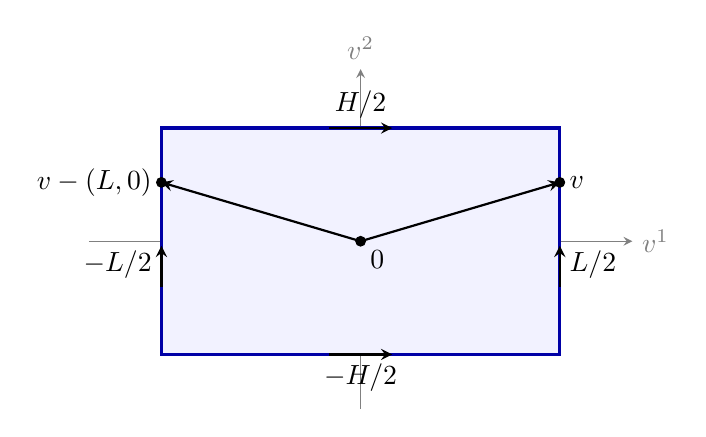
\begin{tikzpicture}[scale=1.15,>=stealth]
	\draw[->,gray] (-3.0,0)--(3.0,0) node[right] {\(v^1\)};
	\draw[->,gray] (0,-1.85)--(0,1.9) node[above] {\(v^2\)};
	\fill[blue!5] (-2.2,-1.25) rectangle (2.2,1.25);
	\draw[very thick,blue!65!black] (-2.2,-1.25) rectangle (2.2,1.25);
	\draw[thick,->] (0,0)--(2.2,0.65);
	\draw[thick,->] (0,0)--(-2.2,0.65);
	\fill (0,0) circle (1.7pt) node[below right] {\(0\)};
	\fill (2.2,0.65) circle (1.7pt) node[right] {\(v\)};
	\fill (-2.2,0.65) circle (1.7pt) node[left] {\(v-(L,0)\)};
	\node[below] at (0,-1.25) {\(-H/2\)};
	\node[above] at (0,1.25) {\(H/2\)};
	\node[below right] at (2.2,0) {\(L/2\)};
	\node[below left] at (-2.2,0) {\(-L/2\)};
	\draw[->,thick] (-0.35,1.25)--(0.35,1.25);
	\draw[->,thick] (-0.35,-1.25)--(0.35,-1.25);
	\draw[->,thick] (2.2,-0.5)--(2.2,-0.05);
	\draw[->,thick] (-2.2,-0.5)--(-2.2,-0.05);
\end{tikzpicture}

	\caption[矩形平坦环面的割迹]{矩形平坦环面的割迹。取格 \(L\mathbb Z\times H\mathbb Z\)，图中矩形为原点的最近点区域 \([-L/2,L/2]\times[-H/2,H/2]\)。相对边在商中识别，整条边界的像组成基点的割迹；边中点有两条最短线，角点有四条。}
	\label{g3:fig:torus-cut-locus}
\end{figure}

覆盖空间也能用来计算其他商度量。下面先把所需的距离公式和完备性传递写清楚。

\begin{proposition}[黎曼覆盖的距离公式]\label{g3:prop:riemannian-covering-distance}
	设 \(\pi:(\widetilde M,\widetilde g)\to(M,g)\) 是连通无边界黎曼流形之间的覆盖，且每点附近的限制是等距映射。若 \(\widetilde M\) 完备，则 \(M\) 完备。对固定提升 \(\widetilde p\in\pi^{-1}(p)\)，有
	\[
		d_M(p,q)=\min_{\widetilde q\in\pi^{-1}(q)}
		d_{\widetilde M}(\widetilde p,\widetilde q).
	\]
	若覆盖来自等距变换群 \(\Gamma\) 的自由作用且纤维正是其轨道，右边等于 \(\min_{\gamma\in\Gamma}d_{\widetilde M}(\widetilde p,\gamma\widetilde q_0)\)，其中 \(\widetilde q_0\) 是任一固定提升。
\end{proposition}
\begin{proof}
	局部等距保持 Levi-Civita 联络：将一个联络通过局部等距搬运，仍满足度量相容和无挠，由唯一性就是另一侧的 Levi-Civita 联络。因此它保持测地线与长度。给定 \(M\) 上的测地线初值，在 \(\widetilde M\) 选取对应初值，所得全时测地线投影后就是原初值的全时解。故 \(M\) 测地完备，再由 Hopf--Rinow 定理得到度量完备。

	在 \(M\) 上取从 \(p\) 到 \(q\) 的最短测地线，从 \(\widetilde p\) 将其提升，终点记为 \(\widetilde q\)。提升长度仍为 \(d_M(p,q)\)，所以 \(d_{\widetilde M}(\widetilde p,\widetilde q)\le d_M(p,q)\)。反向不等式对任意提升终点都成立，因为连接提升端点的曲线投影后长度不变。两者合并，既得到等式，也证明最小值取得。轨道表述只是把纤维中的点重新标记。
\end{proof}

\begin{example}[实射影空间]\label{g3:exm:projective-cut-locus}
	令 \(\mathbb{RP}^n=S_a^n/\{p\sim-p\}\)，取使商映射局部等距的度量。反极点作用自由，足够小的球与其反极点球不交，所以商映射是二重覆盖。令 \(\theta=\arccos(\langle p,q\rangle/a^2)\)，上一命题给出
	\[
		d([p],[q])=a\min\{\theta,\pi-\theta\}
		=a\arccos\frac{|\langle p,q\rangle|}{a^2}.
	\]
	从 \([p]\) 出发的单位速测地线提升为从 \(p\) 出发的大圆；它在 \(t\le\pi a/2\) 时最短，随后一段时间选取反极点提升更短。因此每个方向的割时为 \(\pi a/2\)，割迹为赤道 \(\{q:\langle p,q\rangle=0\}\) 在商中的像，即嵌入的 \(\mathbb{RP}^{n-1}\)。在半径 \(\pi a/2\) 的开切球上，球面指数映射的像是以 \(p\) 为中心的开半球，它与自身的反极点像不交，故商后的指数映射是微分同胚。任意更大的切球内，\((\pi a/2)u\) 与 \(-(\pi a/2)u\) 的像相同，故
	\[
		\operatorname{inj}(\mathbb{RP}^n)=\pi a/2.
	\]
\end{example}

球面在一个点处汇集所有割方向，矩形平坦环面把最近点区域的边界粘成图形，实射影空间则出现整个射影超平面。这些差别来自指数映射的全局行为；点附近总能建立法坐标，并不能决定较远处最短线的条数。
% 纲要条目排为编号小节标题，并进入目录与书签；说明段仍保留于纲要注释中。


\begin{chaptersummary}
	测地线由初始位置和速度唯一确定，速度长度恒定。指数映射把初速度变成时间一的终点；其零处微分为恒等映射，所以零向量附近有法坐标。Gauss 引理进一步说明径向与角向变化正交，从而给出径向线的长度下界及等号条件。出界曲线也必须先付出足够的长度，这使局部计算能够与流形中的所有竞争曲线比较。

	\ProseParagraphBreak

	曲线长度的下确界是与流形拓扑一致的距离。双端点指数映射提供统一的短线，坐标平方函数沿短测地线的凸性则给出强凸邻域。最短曲线不能有角点，按弧长参数化后必为测地线；反过来，一条测地线延长后可能不再最短。

	\ProseParagraphBreak

	Hopf--Rinow 定理把度量完备、所有测地线全时存在、某个基点的指数映射全域定义，以及闭有界集紧性连成等价闭环。完备性还保证任意两点之间存在最短测地线。割时记录这种极小性沿某个方向能保持多久；割时之前的最短线唯一，有限割时处则出现多条最短线或指数映射微分退化。注入半径给出指数坐标可用的球半径，并在紧集上有统一正下界。球面、平坦环面与实射影空间展示了不同的全局识别方式。
\end{chaptersummary}

\BookExercises

\begin{exercise}\label{g3:ex:exponential-line-incomplete}
	在 \(M=\mathbb R\) 上取度量 \(g=e^{2x}\mathrm{d}x^2\)。
	\begin{enumerate}
		\item 证明 \(F(x)=e^x\) 是到 Euclid 半直线 \((0,\infty)\) 的等距微分同胚，并求内在距离 \(d_g(p,q)\)。
		\item 对初值 \(\gamma(0)=p\)、\(\dot\gamma(0)=v\partial_x|_p\)，求最大测地线及其定义区间，进而求 \(\exp_p\) 的定义域和表达式。
		\item 按\cref{g3:def:injectivity-radius}计算 \(\operatorname{inj}_g(p)\)，并证明此流形不完备。
	\end{enumerate}
\end{exercise}
\begin{solution}
	1. \(F\) 是 \(\mathbb R\) 到 \((0,\infty)\) 的光滑双射，其逆为对数函数，且
	\[
		F^*(\mathrm{d}y^2)=(e^x\mathrm{d}x)^2=g.
	\]
	因此它保持曲线长度。半直线内任意连接 \(e^p,e^q\) 的曲线长度至少为 \(|e^q-e^p|\)，连接端点的直线段仍在半直线内并达到这个下界，故
	\[
		d_g(p,q)=|e^q-e^p|.
	\]

	2. 在坐标 \(y=F(x)\) 中，测地线方程是 \(\ddot y=0\)。初速度变为 \(\dot y(0)=e^pv\)，所以
	\[
		y(t)=e^p(1+vt),\qquad
		\gamma(t)=p+\log(1+vt).
	\]
	允许的最大时间区间由 \(1+vt>0\) 决定：
	\[
		I_{p,v}=
		\begin{cases}
			(-1/v,\infty),&v>0,\\
			\mathbb R,&v=0,\\
			(-\infty,-1/v),&v<0.
		\end{cases}
	\]
	有限端点处 \(y(t)\to0\)，对应 \(\gamma(t)\to-\infty\)，没有流形内的延拓点。时间一可取当且仅当 \(v>-1\)，故
	\[
		\mathcal E_p=\{v\partial_x|_p:v>-1\},\qquad
		\exp_p(v\partial_x|_p)=p+\log(1+v).
	\]

	3. 切向量的度量长度为 \(g_p(v\partial_x,v\partial_x)^{1/2}=e^p|v|\)，因而半径 \(r\) 的切球对应区间 \((-re^{-p},re^{-p})\)。当 \(0<r\le e^p\) 时，这个开区间包含于 \(v>-1\)，且指数映射的导数 \(1/(1+v)\) 为正，故指数映射在该球上为微分同胚。若 \(r>e^p\)，切球包含 \(v=-1\)，指数映射在此没有定义。因此
	\[
		\operatorname{inj}_g(p)=e^p.
	\]
	序列 \(p_j=-j\) 关于 \(d_g\) 为 Cauchy 序列，因为 \(F(p_j)=e^{-j}\to0\)；它在 \(M\) 中没有极限。也可以取 \(v=-1\)，得到在时间一终止的最大测地线。这分别检验了度量不完备和测地不完备。
\end{solution}

\begin{exercise}\label{g3:ex:complete-product-distance-injectivity}
	设 \((M,g)\)、\((N,h)\) 为连通、无边界的完备光滑黎曼流形，乘积上取度量 \(G=g\oplus h\)。证明
	\[
		d_G((p,q),(p',q'))^2=d_g(p,p')^2+d_h(q,q')^2,
	\]
	并证明 \(M\times N\) 完备。求乘积的指数映射，再按定义证明
	\[
		\operatorname{inj}_G(p,q)
		=\min\{\operatorname{inj}_g(p),\operatorname{inj}_h(q)\},
	\]
	其中允许半径为无穷。
\end{exercise}
\begin{solution}
	对乘积曲线 \(c=(\alpha,\beta):[0,1]\to M\times N\)，记两个分量的速度长度为 \(a(t),b(t)\)，曲线长度为 \(L_\alpha,L_\beta\)。积分的向量三角不等式给出
	\[
		L_G(c)=\int_0^1\sqrt{a(t)^2+b(t)^2}\,\mathrm{d}t
		\ge\sqrt{L_\alpha^2+L_\beta^2}
		\ge\sqrt{d_g(p,p')^2+d_h(q,q')^2}.
	\]
	第一处不等式也可直接检验：若 \((L_\alpha,L_\beta)\ne(0,0)\)，将 \((a(t),b(t))\) 与其积分向量的单位方向作内积，再逐点用内积不等式，积分即可。零向量情形直接成立。

	由\cref{g3:thm:hopf-rinow}，两个因子中均存在实现端点距离的测地线。将它们都参数化在 \([0,1]\) 上，使速度长度分别恒为 \(d_g(p,p')\)、\(d_h(q,q')\)；距离为零的因子取常曲线。它们组成的乘积曲线速度长度恒为这两个数的平方和开根，达到上述下界。因此距离公式成立。乘积中的 Cauchy 序列投影到两个因子后仍是 Cauchy 序列，各有极限；距离公式又说明乘积序列收敛到两极限组成的点，故乘积完备。

	由\cref{g3:prop:product-connection}，乘积测地线方程分成两个因子的测地线方程，初值唯一性给出
	\[
		\exp^G_{(p,q)}(v,w)
		=(\exp^g_pv,\exp^h_qw),\qquad
		|(v,w)|_G^2=|v|_g^2+|w|_h^2.
	\]
	完备性保证这些指数映射处处有定义。若 \(r\) 小于两个因子的注入半径，则各指数映射在半径 \(r\) 的切球上都是微分同胚，它们的乘积在两个切球的乘积上也是微分同胚。半径 \(r\) 的乘积切球是其中的开子集，故限制后仍为微分同胚，得到所求等式的“\(\ge\)”方向。

	反过来，若乘积指数映射在半径 \(r\) 的切球上为微分同胚，则限制到 \((v,0)\)、\(|v|_g<r\)，可知 \(\exp_p^g\) 在 \(B_p(0,r)\) 上单射。同时
	\[
		\mathrm{d}\exp^G_{(p,q)}\big|_{(v,0)}
		=\operatorname{diag}\bigl((\mathrm{d}\exp^g_p)_v,
			(\mathrm{d}\exp^h_q)_0\bigr)
	\]
	可逆，且第二块为恒等，所以第一块可逆。于是 \(\exp_p^g\) 是单射的局部微分同胚，其局部光滑逆拼成像上的光滑逆；它在整个 \(B_p(0,r)\) 上为微分同胚。交换两个因子，得到同样的结论。故任意乘积可用半径都是两个因子各自的可用半径，对上确界取值即得“\(\le\)”方向，也包括无穷半径的情形。
\end{solution}

\begin{exercise}\label{g3:ex:complete-metric-lower-bound}
	设 \(g,h\) 是同一连通、无边界光滑流形 \(M\) 上的黎曼度量，且 \((M,g)\) 完备。
	\begin{enumerate}
		\item 若存在常数 \(c>0\)，使 \(h(\xi,\xi)\ge c^2g(\xi,\xi)\) 对一切切向量成立，证明 \((M,h)\) 完备。说明仅有距离下界以后，还需怎样把 \(g\) 意义下的极限变成 \(h\) 意义下的极限。
		\item 证明全局上界 \(h\le C^2g\) 不能替代这一假设。可在 \(\mathbb R\) 上取
		\[
			g=\mathrm{d}x^2,\qquad
			h=e^{-2\sqrt{1+x^2}}\mathrm{d}x^2.
		\]
	\end{enumerate}
\end{exercise}
\begin{solution}
	1. 对每条分片光滑曲线积分速度下界，得到 \(L_h\ge cL_g\)，继而
	\[
		d_h(x,y)\ge c\,d_g(x,y).
	\]
	所以 \(h\)-Cauchy 序列 \((p_j)\) 也是 \(g\)-Cauchy 序列。由 \(g\) 完备，存在 \(p\in M\)，使 \(d_g(p_j,p)\to0\)。\cref{g3:thm:riemannian-distance}说明 \(p_j\) 在流形拓扑中也趋于 \(p\)。

	取以 \(p\) 为原点的坐标图，并在其中取闭包紧含于图域的坐标球。度量 \(h\) 的系数在这个闭球上有界，因此存在 \(A>0\)，使 \(h_{ab}(x)\xi^a\xi^b\le A^2|\xi|^2\)。充分大的 \(j\) 位于较小坐标球中，将 \(p_j\) 与 \(p\) 用坐标直线段连接，便有
	\[
		d_h(p_j,p)\le A\,|x(p_j)-x(p)|\longrightarrow0.
	\]
	这一步只在极限点附近使用度量上界；全局不要求 \(h\) 被 \(g\) 的常数倍控制。由此每个 \(h\)-Cauchy 序列都收敛，故 \(h\) 完备。

	2. 所给度量光滑正定，且 \(h\le g\)。令
	\[
		F(x)=\int_0^x e^{-\sqrt{1+s^2}}\,\mathrm{d}s,\qquad
		A=\int_0^\infty e^{-\sqrt{1+s^2}}\,\mathrm{d}s.
	\]
	因 \(\sqrt{1+s^2}\ge s\) 对 \(s\ge0\) 成立，有 \(0<A\le1\)。\(F'\) 处处为正，且被积函数为偶函数，所以 \(F\) 是到有限开区间 \((-A,A)\) 的微分同胚，满足 \(F^*(\mathrm{d}y^2)=h\)。因此
	\[
		d_h(x,y)=|F(x)-F(y)|.
	\]
	序列 \(x_j=j\) 映到趋于 \(A\) 的序列，是 \(h\)-Cauchy 序列，却没有流形内的极限。缩小远处的长度尺度可以使通往无穷远的路径具有有限长度，因此全局上界 \(h\le g\) 不能保证完备性。
\end{solution}

\begin{exercise}\label{g3:ex:squared-distance-at-center}
	设 \((M,g)\) 为无边界光滑黎曼流形，\(\exp_p:B_p(0,R)\to U_R\) 为微分同胚，令 \(r(q)=d_g(p,q)\)。证明 \(r\) 在 \(U_R\setminus\{p\}\) 上光滑，并求其梯度，证明 \(|\operatorname{grad}_g r|_g=1\)。再证明 \(f=r^2\) 在整个 \(U_R\) 上光滑，且
	\[
		(H_f)_p=2g_p.
	\]
	这里沿用协变二阶导数的定义
	\[
		H_f(X,Y)=X(Yf)-(\nabla_XY)f.
	\]
\end{exercise}
\begin{solution}
	由\cref{g3:prop:normal-radial-minimality}，若 \(q=\exp_p(v)\)，则 \(r(q)=|v|_g\)。因此 \(r\) 在去掉中心的法邻域中光滑。固定非零 \(v\)，令 \(u=v/|v|_g\)。对任意 \(w\in\mathrm{T}_pM\)，有
	\[
		\mathrm{d}r_q\bigl((\mathrm{d}\exp_p)_vw\bigr)
		=\frac{g_p(v,w)}{|v|_g}.
	\]
	Gauss 引理把右端改写为
	\[
		g_q\bigl((\mathrm{d}\exp_p)_vu,(\mathrm{d}\exp_p)_vw\bigr).
	\]
	由于 \((\mathrm{d}\exp_p)_v\) 可逆，这对 \(q\) 处的全部切向量确定了梯度：
	\[
		\operatorname{grad}_g r\big|_q=(\mathrm{d}\exp_p)_vu=\partial_r|_q,
		\qquad |\operatorname{grad}_g r|_g=1.
	\]

	取由 \(\mathrm{T}_pM\) 的正交单位基得到的法坐标，则
	\[
		f(x)=r(x)^2=\sum_i(x^i)^2.
	\]
	此表达在中心也光滑，且 \(\mathrm{d}f_p=0\)。由 \(H_f\) 的定义直接得到坐标分量
	\[
		(H_f)_{ij}=\partial_i\partial_jf-\Gamma^k_{ij}\partial_kf.
	\]
	在 \(p\) 处第二项为零，第一项是 \(2\delta_{ij}\)。又 \(g_{ij}(p)=\delta_{ij}\)，故 \((H_f)_p=2g_p\)。距离函数本身在中心有绝对值型行为，平方则消除了这一不可微点。
\end{solution}

\begin{exercise}\label{g3:ex:completeness-escaping-curves}
	设 \((M,g)\) 为连通、无边界光滑黎曼流形。称连续曲线 \(c:[0,b)\to M\)、\(0<b\le\infty\)，在 \(t\uparrow b\) 时离开所有紧集，是指对每个紧集 \(K\subset M\)，都存在 \(t_K<b\)，使 \(c(t)\notin K\) 对 \(t_K<t<b\) 成立。假设曲线在每个紧参数子区间上分片光滑，并定义
	\[
		L_g(c)=\sup_{0<T<b}L_g(c|_{[0,T]}).
	\]
	证明：\(M\) 完备，当且仅当每条离开所有紧集的这种曲线都有无限长度。反向证明中，可使用有限端点的最大测地线，但须证明其位置确实离开所有紧集。
\end{exercise}
\begin{solution}
	先设 \(M\) 完备。若某条曲线的总长度为有限数 \(L\)，则对所有 \(t<b\)，
	\[
		d_g(c(0),c(t))\le L.
	\]
	由 Hopf--Rinow 定理，闭距离球 \(\overline B_{d_g}(c(0),L)\) 紧，而整条曲线都在其中。因此它不能离开所有紧集，证明一个方向。

	反过来，若 \(M\) 不完备，Hopf--Rinow 定理给出一条不能全时延拓的最大测地线。必要时反向并作仿射重参数化，可取单位速测地线 \(\gamma:[0,b)\to M\)，其中 \(b<\infty\) 是其最大右端点。它的长度为 \(b\)。下面证明它离开所有紧集。

	若存在紧集 \(K\) 和时刻 \(t_j\uparrow b\)，使 \(\gamma(t_j)\in K\)，取子列可使 \(\gamma(t_j)\to q\in K\)。因速度为一，当 \(t<t_j\) 时有
	\[
		d_g(\gamma(t),\gamma(t_j))\le t_j-t.
	\]
	让 \(j\to\infty\)，得到 \(d_g(\gamma(t),q)\le b-t\)，所以整个曲线尾部趋于 \(q\)。这里从反复进入紧集到存在位置极限，使用了有限剩余长度；仅知道测地线的某些位置有收敛子列尚不足以直接给出二阶方程的初值。

	在 \(q\) 附近取闭包紧含于一个坐标图的邻域，曲线尾部最终留在其中。度量矩阵有统一正下界，因此单位速条件使坐标速度 \(\dot x(t)\) 有界；Christoffel 系数也有界，由
	\[
		\ddot x^k=-\Gamma^k_{ij}(x)\dot x^i\dot x^j
	\]
	可知坐标加速度有界。于是 \(\dot x(t)\) 在 \(t\uparrow b\) 时有极限 \(w\)，并且 \((x(t),\dot x(t))\to(x(q),w)\)。测地线一阶系统的积分形式延续到 \(b\)；以 \((q,w)\) 为初值应用\cref{g3:thm:geodesic-ivp}，便将原解延长到 \(b\) 之后，违背最大性。因此每个紧集都只能在某个末时刻以前被访问，\(\gamma\) 确实离开所有紧集。它具有有限长度，与题设性质矛盾，故该性质推出完备。
\end{solution}

\begin{exercise}\label{g3:ex:sphere-normal-volume}
	在半径 \(a>0\) 的圆球面 \(S_a^n\subset\mathbb R^{n+1}\)、\(n\ge1\) 上，固定 \(p\) 并使用由 \(\mathrm{T}_pS_a^n\) 的正交单位基产生的法坐标。设 \(v=ru\)、\(0<r<\pi a\)、\(|u|=1\)。直接对式\eqref{g3:eq:round-sphere-exponential}求微分，证明 \(\exp_p\) 在径向上的长度倍率为 \(1\)，在与 \(v\) 正交的方向上的长度倍率为
	\[
		s(r)=\frac{\sin(r/a)}{r/a}.
	\]
	由此求法坐标中的度量矩阵及体积密度，并说明其在中心的延拓。
\end{exercise}
\begin{solution}
	对任意 \(w\in\mathrm{T}_pS_a^n\)，写
	\[
		w=\lambda u+w_\perp,\qquad
		\lambda=\langle u,w\rangle,\quad w_\perp\perp u.
	\]
	因为 \(\mathrm{d}r_v(w)=\lambda\)、\(\mathrm{d}u_v(w)=w_\perp/r\)，对
	\[
		\exp_p(v)=\cos(r/a)p+a\sin(r/a)u
	\]
	求微分得到
	\[
		(\mathrm{d}\exp_p)_vw
		=\lambda E_r+s(r)w_\perp,\qquad
		E_r=-\frac{\sin(r/a)}a\,p+\cos(r/a)u.
	\]
	向量 \(E_r\) 的环境长度为一，并且与 \(w_\perp\) 正交；两者都切于终点球面。因此
	\[
		\left|(\mathrm{d}\exp_p)_vw\right|_g^2
		=\lambda^2+s(r)^2|w_\perp|^2,
	\]
	给出两种所求倍率。这个计算还直接验证了 Gauss 引理中的径向正交性。

	在固定正交单位基中写 \(v=(x^1,\ldots,x^n)\)，则 \(r^2=\sum_i(x^i)^2\)，拉回度量矩阵为
	\[
		g_{ij}(x)=s(r)^2\delta_{ij}
		+\bigl(1-s(r)^2\bigr)\frac{x^ix^j}{r^2}.
	\]
	径向特征值为 \(1\)，其余 \(n-1\) 个特征值为 \(s(r)^2\)。在 \(0<r<\pi a\) 内，\(s(r)>0\)，所以
	\[
		\sqrt{\det(g_{ij}(x))}
		=s(r)^{n-1},\qquad
		\mu_g=
		\left(\frac{\sin(r/a)}{r/a}\right)^{n-1}
		\left|\mathrm{d}x^1\cdots\mathrm{d}x^n\right|.
	\]
	当 \(n=1\) 时没有横向方向，密度系数为 \(1\)，与此公式一致。

	最后，\(\sin z/z\) 在 \(z=0\) 的值取 \(1\) 后，是 \(z^2\) 的光滑函数。因而 \(s(r)\) 是 \(r^2\) 的光滑函数，且
	\[
		s(r)^2=1-\frac{r^2}{3a^2}+O(r^4).
	\]
	于是 \((1-s(r)^2)/r^2\) 在零处光滑延拓，取值为 \(1/(3a^2)\)；度量矩阵在中心延拓为 \(\delta_{ij}\)，体积密度系数光滑延拓为 \(1\)。以上计算直接使用显式指数映射，给出了正曲率球面相对于切空间 Euclid 体积的局部变化。
\end{solution}

\begin{exercise}\label{g3:ex:rectangular-torus-distance}
	设 \(T=\mathbb R^2/(L\mathbb Z\times H\mathbb Z)\)，其中 \(L,H>0\)，取平坦商度量。计算其直径、注入半径，以及从原点类到任意一点的最短测地线条数。再考虑平坦圆柱 \(C=\mathbb R\times(\mathbb R/L\mathbb Z)\)，求原点类的割迹和单位方向 \(u=(u_1,u_2)\) 的割时。
\end{exercise}
\begin{solution}
	每个点类都有代表 \((x,y)\in[-L/2,L/2]\times[-H/2,H/2]\)。由式\eqref{g3:eq:flat-torus-distance}，到原点类的距离为 \(\sqrt{x^2+y^2}\)，故最大值在角点取得，为 \(\tfrac12\sqrt{L^2+H^2}\)。平移是等距映射，所以任意点对的距离也不超过此值，从而
	\[
		\operatorname{diam}(T)=\tfrac12\sqrt{L^2+H^2},\qquad
		\operatorname{inj}(T)=\tfrac12\min\{L,H\}.
	\]
	最近代表在每个坐标方向独立选择：若 \(|x|<L/2\)，第一个坐标唯一；若 \(|x|=L/2\)，两个符号都可选。第二个坐标同理。因此最近点区域内部的点有一条最短线，边的内部有两条，四角共同代表的点有四条。从基点到自身，最短线只有常值曲线。每个最近代表给出一个直线段，其投影的初速度不同，故这些线确实互不相同；任意最短线提升后又必须是到某个最近代表的直线段，所以没有遗漏。

	圆柱只在第二坐标上取商，距离公式为
	\[
		d_C([0,0],[x,y])=\min_{k\in\mathbb Z}\sqrt{x^2+(y+kL)^2}.
	\]
	最近点区域是无限条带 \(|y|\le L/2\)，两条边界在商中识别，故原点类的割迹为直线 \(\{[x,L/2]:x\in\mathbb R\}\)。沿方向 \(u\) 的线最短恰好到第一次抵达该边界，因此
	\[
		c_p(u)=
		\begin{cases}
			L/(2|u_2|),&u_2\ne0,\\
			\infty,&u_2=0.
		\end{cases}
	\]
	相应注入半径为 \(L/2\)。同一个完备流形上，可以有永远最短的方向，也可以有有限割时的方向。
\end{solution}

\begin{exercise}\label{g3:ex:complete-cusp-zero-injectivity}
	设 \((M,g)\) 连通、完备、无边界。
	\begin{enumerate}
		\item 若基于 \(p\) 的分片光滑环路 \(\alpha\) 不能在 \(M\) 中收缩为常值环路，证明 \(\operatorname{inj}_g(p)\le L_g(\alpha)/2\)。
		\item 在圆柱 \(M=\mathbb R\times(\mathbb R/2\pi\mathbb Z)\) 上取
		\[
			g=\mathrm dr^2+e^{-2r}\mathrm d\theta^2.
		\]
		证明它完备，但 \(\operatorname{inj}_g(M)=0\)。
	\end{enumerate}
\end{exercise}
\begin{solution}
	1. 记 \(\ell=L_g(\alpha)\)。沿环路的正向和反向两段都能连接 \(p\) 与任意一点 \(q\)，其中较短的一段长至多 \(\ell/2\)，所以整条环路位于 \(\overline B_d(p,\ell/2)\)。若 \(\ell/2<\operatorname{inj}_g(p)\)，取
	\[
		\ell/2<\rho<\operatorname{inj}_g(p).
	\]
	由\cref{g3:prop:compact-injectivity-lower-bound}，\(B_d(p,\rho)=\exp_p B_p(0,\rho)\)，且指数映射是微分同胚。于是
	\[
		H(s,t)=\exp_p\bigl((1-s)\exp_p^{-1}\alpha(t)\bigr)
	\]
	在固定基点的条件下把 \(\alpha\) 收缩为常值环路，矛盾。

	2. 对任意连接曲线，都有 \(L_g\ge\int|\dot r|\)，因此 \(|r-r'|\le d_g((r,\theta),(r',\theta'))\)。若 \((r_j,\theta_j)\) 为 Cauchy 序列，\(r_j\) 为实数 Cauchy 序列，特别地全部落在某个有界闭区间 \([A,B]\) 中。拓扑圆柱带 \([A,B]\times S^1\) 紧，故该序列有子列在流形拓扑中收敛；距离拓扑相同，所以此子列也在 \(d_g\) 下收敛。Cauchy 性再使整个序列收敛，证明完备。

	基于 \(p_r=(r,0)\) 的圆周环路 \(\alpha_r(t)=(r,2\pi t)\) 长为 \(2\pi e^{-r}\)，且不可收缩。事实上，若它可收缩，投影到第二因子就会把圆周绕行一周的环路收缩；在覆盖 \(\mathbb R\to S^1\)、\(s\mapsto e^{is}\) 下，该环路从零出发的提升终止于 \(2\pi\)，而常值环路的提升终止于零，与第一卷第5.3节的定端点同伦提升结论矛盾。由第一问，
	\[
		0<\operatorname{inj}_g(p_r)\le\pi e^{-r}.
	\]
	令 \(r\to+\infty\)，得到整体下确界为零。各点的注入半径仍为正，趋于零发生在离开所有紧集的过程中。
\end{solution}

\begin{exercise}\label{g3:ex:covering-completeness-converse}
	设 \(\pi:(\widetilde M,\widetilde g)\to(M,g)\) 是连通无边界黎曼流形之间的覆盖，且处处局部等距。证明 \(M\) 完备当且仅当 \(\widetilde M\) 完备。给出一个局部等距映射，说明删去覆盖条件后，从目标完备不能推出源完备。
\end{exercise}
\begin{solution}
	从源完备推出目标完备已由\cref{g3:prop:riemannian-covering-distance}证明。反过来设 \(M\) 完备，给定 \(\widetilde M\) 上的初值 \((\widetilde p,\widetilde v)\)。将其投影到 \(M\)，所得测地线 \(\gamma\) 定义在整个实轴上。对每个正整数 \(N\)，在 \([-N,N]\) 上从 \(t=0\) 分别向正负方向提升 \(\gamma\)，初点指定为 \(\widetilde p\)。道路提升唯一性保证不同 \(N\) 的提升在公共区间相等，因而拼成 \(\mathbb R\) 上的一条提升 \(\widetilde\gamma\)。局部覆盖逆为等距映射，所以提升光滑，并保持测地线方程；其初速度就是 \(\widetilde v\)。由此全部测地线初值全时可解，Hopf--Rinow 定理给出 \(\widetilde M\) 完备。

	带普通度量的包含映射 \((0,1)\hookrightarrow\mathbb R\) 局部等距，但目标完备而源不完备。有限时间内，源中的直线可以到达被删去的端点；该映射不是到 \(\mathbb R\) 的覆盖，不能对全时的目标直线作所需提升。
\end{solution}

\begin{exercise}\label{g3:ex:noncompact-complete-ray}
	设 \((M,g)\) 连通、完备、无边界且非紧。证明对任意 \(p\in M\)，存在单位速测地线 \(\gamma:[0,\infty)\to M\)，满足
	\[
		d(\gamma(s),\gamma(t))=t-s\qquad(0\le s\le t).
	\]
	这样的曲线称为从 \(p\) 出发的测地射线。由此证明至少存在一个 \(u\in S_pM\)，使 \(c_p(u)=\infty\)。
\end{exercise}
\begin{solution}
	由 Hopf--Rinow 定理，有限半径闭球紧。若 \(d(p,\cdot)\) 有上界，整个流形就是一个紧闭球，与非紧性矛盾。因此可选 \(q_j\)，使 \(\ell_j=d(p,q_j)\to\infty\)。取从 \(p\) 到 \(q_j\) 的单位速最短测地线，初方向记为 \(u_j\in S_pM\)。有限维单位球面紧，故取子列可使 \(u_j\to u\)。完备性保证 \(\gamma(t)=\exp_p(tu)\) 对所有 \(t\ge0\) 有定义。

	固定 \(0\le s\le t\)。充分大的 \(j\) 有 \(\ell_j\ge t\)，最短线的子段仍最短，故
	\[
		d(\exp_p(su_j),\exp_p(tu_j))=t-s.
	\]
	指数映射和距离均连续，令 \(j\to\infty\) 得到所求等式。取 \(s=0\)，可见从 \(p\) 到 \(\gamma(t)\) 的线段对每个 \(t\) 都最短，所以 \(c_p(u)=\infty\)。
\end{solution}

\begin{exercise}\label{g3:ex:isometry-first-jet}
	设 \(F:(M,g)\to(N,h)\) 为黎曼等距同构，即满足 \(F^*h=g\) 的微分同胚。证明在指数映射有定义处，
	\[
		F(\exp_pv)=\exp_{F(p)}((\mathrm dF)_pv).
	\]
	若 \(M\) 还连通、完备，证明 \(F\) 由一点处的值 \(F(p)\) 及微分 \((\mathrm dF)_p\) 唯一确定。并证明
	\[
		F(\operatorname{Cut}_M(p))=\operatorname{Cut}_N(F(p)),\qquad
		\operatorname{inj}_h(F(p))=\operatorname{inj}_g(p).
	\]
\end{exercise}
\begin{solution}
	将 \(M\) 上的联络通过 \(F\) 搬到 \(N\)，度量相容和无挠性质保持成立，所以它由 Levi-Civita 唯一性就是 \(N\) 上的联络。因此 \(F\circ\gamma_{p,v}\) 是初值 \((F(p),(\mathrm dF)_pv)\) 的测地线。初值唯一性给出全时间的对应，取时间一即得指数映射公式。

	若另一个等距同构 \(G:M\to N\) 在 \(p\) 处有同样的值与微分，则对每个 \(v\in\mathrm T_pM\)，有 \(F(\exp_pv)=G(\exp_pv)\)。Hopf--Rinow 定理使 \(\exp_p\) 满射，所以 \(F=G\) 于整个 \(M\)。

	等距同构保持全部曲线长度与端点距离，其微分把单位切球面等距地对应起来。因此
	\[
		c_{F(p)}((\mathrm dF)_pu)=c_p(u),
	\]
	并把有限割时的终点一一对应，得到割迹等式。指数映射公式还说明，两侧指数映射分别通过线性等距同构 \((\mathrm dF)_p\) 和微分同胚 \(F\) 共轭，所以使指数映射在切球上成为微分同胚的半径完全相同，注入半径相等。
\end{solution}

\begin{exercise}\label{g3:ex:scaling-cut-injectivity}
	设 \((M,g)\) 连通、完备、无边界，\(a>0\)，令 \(\widetilde g=a^2g\)。比较两种度量的距离、指数映射、割迹、割时及注入半径。写出割时公式时，明确两侧单位初方向的对应。
\end{exercise}
\begin{solution}
	每条曲线的长度乘以 \(a\)，取下确界得到 \(d_{\widetilde g}=a\,d_g\)，所以完备性保持不变。上一章的常数缩放计算说明两种度量的 Levi-Civita 联络相同，故同一个切向量给出同一个带参数测地线，指数映射也相同。

	若 \(|u|_g=1\)，则 \(|u/a|_{\widetilde g}=1\)，且
	\[
		d_{\widetilde g}\bigl(p,\exp_p(tu/a)\bigr)
		=a\,d_g\bigl(p,\exp_p((t/a)u)\bigr).
	\]
	左边等于 \(t\)，当且仅当右侧原距离等于 \(t/a\)。因此
	\[
		c_p^{\widetilde g}(u/a)=a\,c_p^g(u).
	\]
	达到有限割时的向量相同：\((a c_p^g(u))(u/a)=c_p^g(u)u\)，所以割迹作为点集不变。最后，\(\widetilde g\) 的半径 \(r\) 切球就是 \(g\) 的半径 \(r/a\) 切球，指数映射本身不变，故
	\[
		\operatorname{inj}_{\widetilde g}(p)=a\,\operatorname{inj}_g(p),\qquad
		\operatorname{inj}_{\widetilde g}(M)=a\,\operatorname{inj}_g(M).
	\]
\end{solution}
